\documentclass[1p]{elsarticle_modified}
%\bibliographystyle{elsarticle-num}

%\usepackage[colorlinks]{hyperref}
%\usepackage{abbrmath_seonhwa} %\Abb, \Ascr, \Acal ,\Abf, \Afrak
\usepackage{amsfonts}
\usepackage{amssymb}
\usepackage{amsmath}
\usepackage{amsthm}
\usepackage{scalefnt}
\usepackage{amsbsy}
\usepackage{kotex}
\usepackage{caption}
\usepackage{subfig}
\usepackage{color}
\usepackage{graphicx}
\usepackage{xcolor} %% white, black, red, green, blue, cyan, magenta, yellow
\usepackage{float}
\usepackage{setspace}
\usepackage{hyperref}

\usepackage{tikz}
\usetikzlibrary{arrows}

\usepackage{multirow}
\usepackage{array} % fixed length table
\usepackage{hhline}

%%%%%%%%%%%%%%%%%%%%%
\makeatletter
\renewcommand*\env@matrix[1][\arraystretch]{%
	\edef\arraystretch{#1}%
	\hskip -\arraycolsep
	\let\@ifnextchar\new@ifnextchar
	\array{*\c@MaxMatrixCols c}}
\makeatother %https://tex.stackexchange.com/questions/14071/how-can-i-increase-the-line-spacing-in-a-matrix
%%%%%%%%%%%%%%%

\usepackage[normalem]{ulem}

\newcommand{\msout}[1]{\ifmmode\text{\sout{\ensuremath{#1}}}\else\sout{#1}\fi}
%SOURCE: \msout is \stkout macro in https://tex.stackexchange.com/questions/20609/strikeout-in-math-mode

\newcommand{\cancel}[1]{
	\ifmmode
	{\color{red}\msout{#1}}
	\else
	{\color{red}\sout{#1}}
	\fi
}

\newcommand{\add}[1]{
	{\color{blue}\uwave{#1}}
}

\newcommand{\replace}[2]{
	\ifmmode
	{\color{red}\msout{#1}}{\color{blue}\uwave{#2}}
	\else
	{\color{red}\sout{#1}}{\color{blue}\uwave{#2}}
	\fi
}

\newcommand{\Sol}{\mathcal{S}} %segment
\newcommand{\D}{D} %diagram
\newcommand{\A}{\mathcal{A}} %arc


%%%%%%%%%%%%%%%%%%%%%%%%%%%%%5 test

\def\sl{\operatorname{\textup{SL}}(2,\Cbb)}
\def\psl{\operatorname{\textup{PSL}}(2,\Cbb)}
\def\quan{\mkern 1mu \triangleright \mkern 1mu}

\theoremstyle{definition}
\newtheorem{thm}{Theorem}[section]
\newtheorem{prop}[thm]{Proposition}
\newtheorem{lem}[thm]{Lemma}
\newtheorem{ques}[thm]{Question}
\newtheorem{cor}[thm]{Corollary}
\newtheorem{defn}[thm]{Definition}
\newtheorem{exam}[thm]{Example}
\newtheorem{rmk}[thm]{Remark}
\newtheorem{alg}[thm]{Algorithm}

\newcommand{\I}{\sqrt{-1}}
\begin{document}

%\begin{frontmatter}
%
%\title{Boundary parabolic representations of knots up to 8 crossings}
%
%%% Group authors per affiliation:
%\author{Yunhi Cho} 
%\address{Department of Mathematics, University of Seoul, Seoul, Korea}
%\ead{yhcho@uos.ac.kr}
%
%
%\author{Seonhwa Kim} %\fnref{s_kim}}
%\address{Center for Geometry and Physics, Institute for Basic Science, Pohang, 37673, Korea}
%\ead{ryeona17@ibs.re.kr}
%
%\author{Hyuk Kim}
%\address{Department of Mathematical Sciences, Seoul National University, Seoul 08826, Korea}
%\ead{hyukkim@snu.ac.kr}
%
%\author{Seokbeom Yoon}
%\address{Department of Mathematical Sciences, Seoul National University, Seoul, 08826,  Korea}
%\ead{sbyoon15@snu.ac.kr}
%
%\begin{abstract}
%We find all boundary parabolic representation of knots up to 8 crossings.
%
%\end{abstract}
%\begin{keyword}
%    \MSC[2010] 57M25 
%\end{keyword}
%
%\end{frontmatter}

%\linenumbers
%\tableofcontents
%
\newcommand\colored[1]{\textcolor{white}{\rule[-0.35ex]{0.8em}{1.4ex}}\kern-0.8em\color{red} #1}%
%\newcommand\colored[1]{\textcolor{white}{ #1}\kern-2.17ex	\textcolor{white}{ #1}\kern-1.81ex	\textcolor{white}{ #1}\kern-2.15ex\color{red}#1	}

{\Large $\underline{12a_{1101}~(K12a_{1101})}$}

\setlength{\tabcolsep}{10pt}
\renewcommand{\arraystretch}{1.6}
\vspace{1cm}\begin{tabular}{m{100pt}>{\centering\arraybackslash}m{274pt}}
\multirow{5}{120pt}{
	\centering
	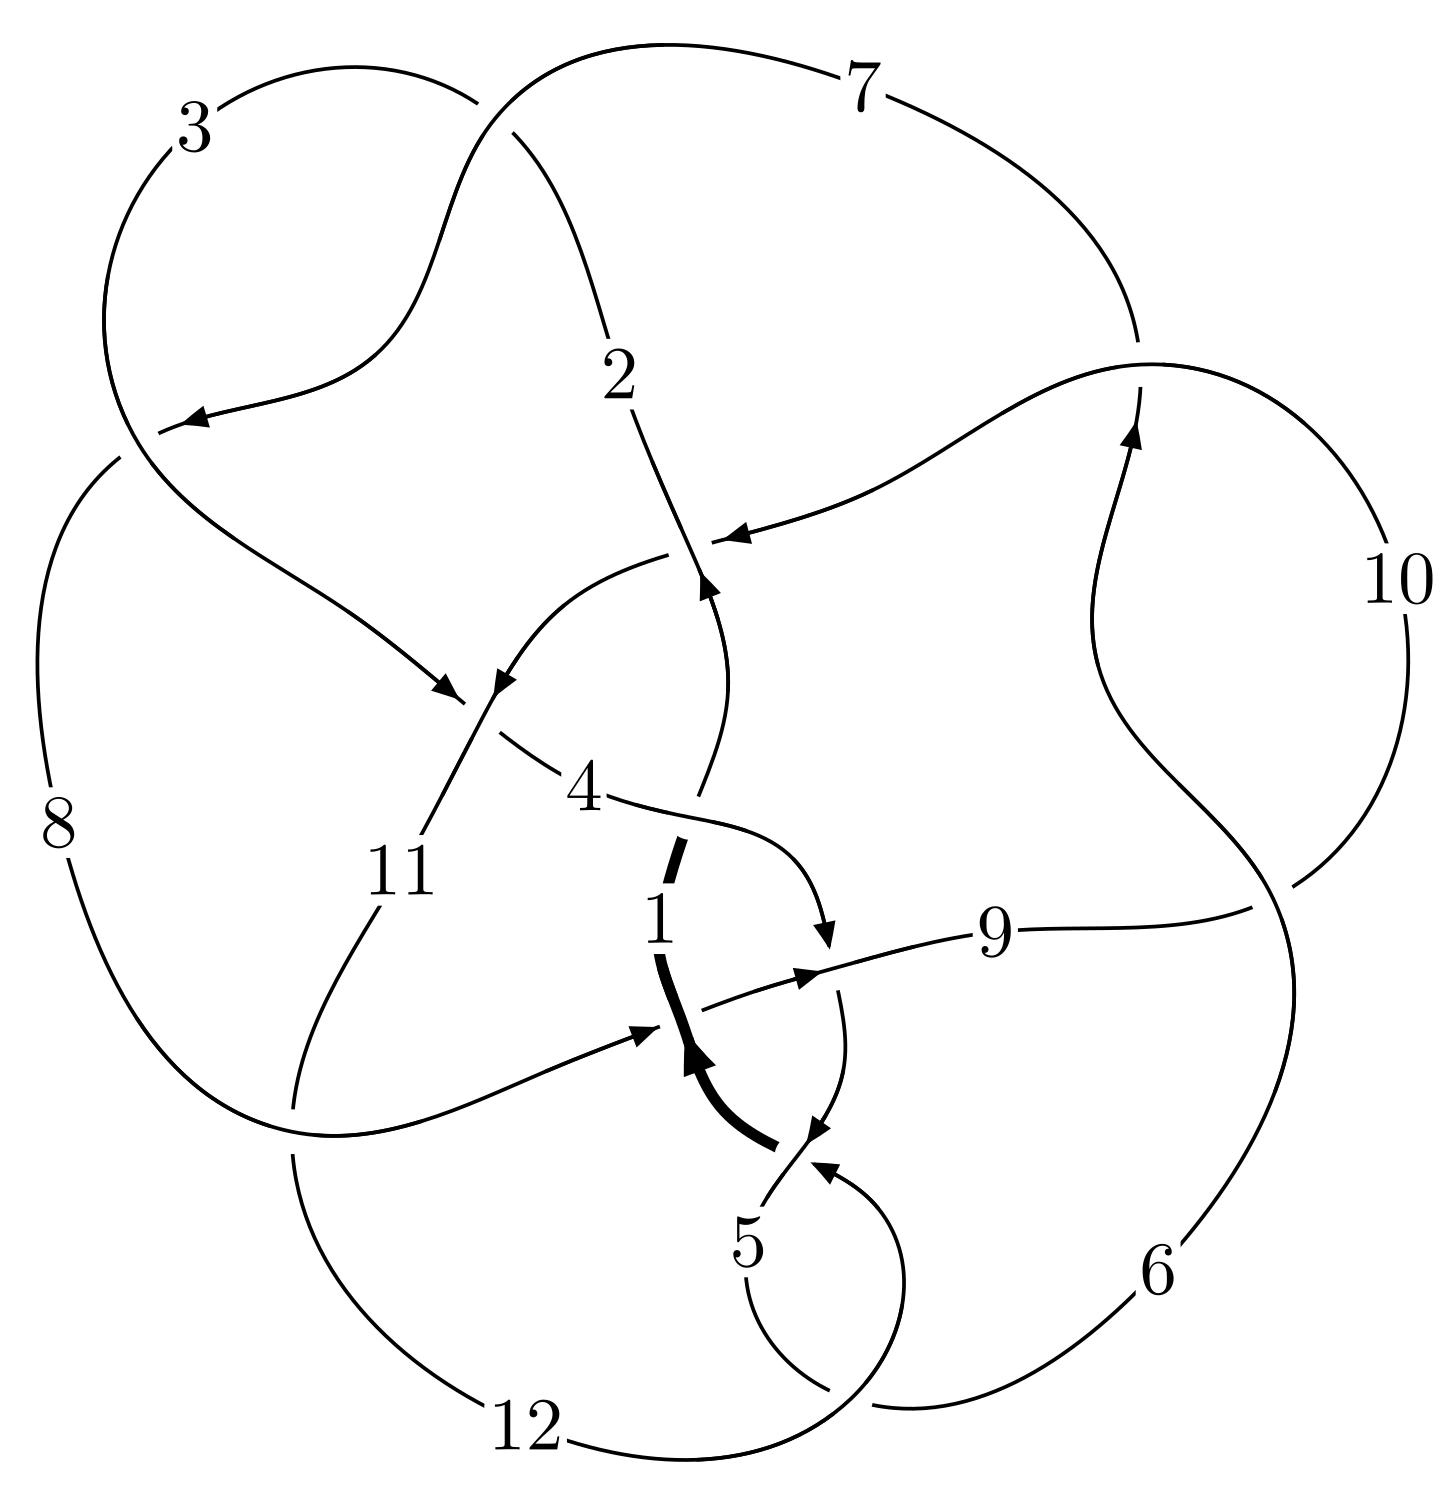
\includegraphics[width=112pt]{../../../GIT/diagram.site/Diagrams/png/1902_12a_1101.png}\\
\ \ \ A knot diagram\footnotemark}&
\allowdisplaybreaks
\textbf{Linearized knot diagam} \\
\cline{2-2}
 &
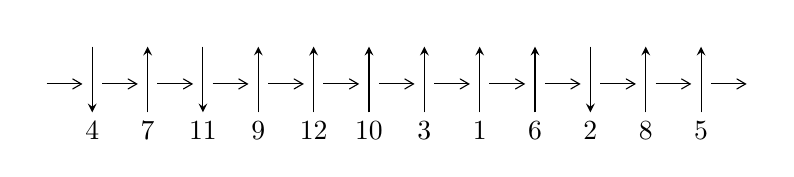
\begin{tikzpicture}[x=20pt, y=17pt]
	% nodes
	\node (C0) at (0, 0) {};
	\node (C1) at (1, 0) {};
	\node (C1U) at (1, +1) {};
	\node (C1D) at (1, -1) {4};

	\node (C2) at (2, 0) {};
	\node (C2U) at (2, +1) {};
	\node (C2D) at (2, -1) {7};

	\node (C3) at (3, 0) {};
	\node (C3U) at (3, +1) {};
	\node (C3D) at (3, -1) {11};

	\node (C4) at (4, 0) {};
	\node (C4U) at (4, +1) {};
	\node (C4D) at (4, -1) {9};

	\node (C5) at (5, 0) {};
	\node (C5U) at (5, +1) {};
	\node (C5D) at (5, -1) {12};

	\node (C6) at (6, 0) {};
	\node (C6U) at (6, +1) {};
	\node (C6D) at (6, -1) {10};

	\node (C7) at (7, 0) {};
	\node (C7U) at (7, +1) {};
	\node (C7D) at (7, -1) {3};

	\node (C8) at (8, 0) {};
	\node (C8U) at (8, +1) {};
	\node (C8D) at (8, -1) {1};

	\node (C9) at (9, 0) {};
	\node (C9U) at (9, +1) {};
	\node (C9D) at (9, -1) {6};

	\node (C10) at (10, 0) {};
	\node (C10U) at (10, +1) {};
	\node (C10D) at (10, -1) {2};

	\node (C11) at (11, 0) {};
	\node (C11U) at (11, +1) {};
	\node (C11D) at (11, -1) {8};

	\node (C12) at (12, 0) {};
	\node (C12U) at (12, +1) {};
	\node (C12D) at (12, -1) {5};
	\node (C13) at (13, 0) {};

	% arrows
	\draw[->,>={angle 60}]
	(C0) edge (C1) (C1) edge (C2) (C2) edge (C3) (C3) edge (C4) (C4) edge (C5) (C5) edge (C6) (C6) edge (C7) (C7) edge (C8) (C8) edge (C9) (C9) edge (C10) (C10) edge (C11) (C11) edge (C12) (C12) edge (C13) ;	\draw[->,>=stealth]
	(C1U) edge (C1D) (C2D) edge (C2U) (C3U) edge (C3D) (C4D) edge (C4U) (C5D) edge (C5U) (C6D) edge (C6U) (C7D) edge (C7U) (C8D) edge (C8U) (C9D) edge (C9U) (C10U) edge (C10D) (C11D) edge (C11U) (C12D) edge (C12U) ;
	\end{tikzpicture} \\
\hhline{~~} \\& 
\textbf{Solving Sequence} \\ \cline{2-2} 
 &
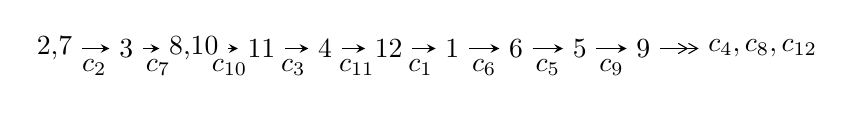
\begin{tikzpicture}[x=23pt, y=7pt]
	% node
	\node (A0) at (-1/8, 0) {2,7};
	\node (A1) at (1, 0) {3};
	\node (A2) at (33/16, 0) {8,10};
	\node (A3) at (25/8, 0) {11};
	\node (A4) at (33/8, 0) {4};
	\node (A5) at (41/8, 0) {12};
	\node (A6) at (49/8, 0) {1};
	\node (A7) at (57/8, 0) {6};
	\node (A8) at (65/8, 0) {5};
	\node (A9) at (73/8, 0) {9};
	\node (C1) at (1/2, -1) {$c_{2}$};
	\node (C2) at (3/2, -1) {$c_{7}$};
	\node (C3) at (21/8, -1) {$c_{10}$};
	\node (C4) at (29/8, -1) {$c_{3}$};
	\node (C5) at (37/8, -1) {$c_{11}$};
	\node (C6) at (45/8, -1) {$c_{1}$};
	\node (C7) at (53/8, -1) {$c_{6}$};
	\node (C8) at (61/8, -1) {$c_{5}$};
	\node (C9) at (69/8, -1) {$c_{9}$};
	\node (A10) at (11, 0) {$c_{4},c_{8},c_{12}$};

	% edge
	\draw[->,>=stealth]	
	(A0) edge (A1) (A1) edge (A2) (A2) edge (A3) (A3) edge (A4) (A4) edge (A5) (A5) edge (A6) (A6) edge (A7) (A7) edge (A8) (A8) edge (A9) ;
	\draw[->>,>={angle 60}]	
	(A9) edge (A10);
\end{tikzpicture} \\ 

\end{tabular} \\

\footnotetext{
The image of knot diagram is generated by the software ``\textbf{Draw programme}" developed by Andrew Bartholomew(\url{http://www.layer8.co.uk/maths/draw/index.htm\#Running-draw}), where we modified some parts for our purpose(\url{https://github.com/CATsTAILs/LinksPainter}).
}\phantom \\ \newline 
\centering \textbf{Ideals for irreducible components\footnotemark of $X_{\text{par}}$} 
 
\begin{align*}
I^u_{1}&=\langle 
4.20156\times10^{826} u^{157}-1.46744\times10^{828} u^{156}+\cdots+7.17053\times10^{829} b-9.65577\times10^{830},\\
\phantom{I^u_{1}}&\phantom{= \langle  }2.89627\times10^{830} u^{157}-3.51152\times10^{830} u^{156}+\cdots+9.35037\times10^{831} a-3.38511\times10^{833},\\
\phantom{I^u_{1}}&\phantom{= \langle  }u^{158}- u^{157}+\cdots-2697 u-163\rangle \\
I^u_{2}&=\langle 
8.79895\times10^{26} u^{39}-1.14601\times10^{27} u^{38}+\cdots+7.82938\times10^{24} b+6.82482\times10^{26},\\
\phantom{I^u_{2}}&\phantom{= \langle  }3.10296\times10^{27} u^{39}-4.02963\times10^{27} u^{38}+\cdots+1.56588\times10^{25} a+2.38940\times10^{27},\;u^{40}-11 u^{38}+\cdots+2 u+1\rangle \\
\\
\end{align*}
\raggedright * 2 irreducible components of $\dim_{\mathbb{C}}=0$, with total 198 representations.\\
\footnotetext{All coefficients of polynomials are rational numbers. But the coefficients are sometimes approximated in decimal forms when there is not enough margin.}
\newpage
\renewcommand{\arraystretch}{1}
\centering \section*{I. $I^u_{1}= \langle 4.20\times10^{826} u^{157}-1.47\times10^{828} u^{156}+\cdots+7.17\times10^{829} b-9.66\times10^{830},\;2.90\times10^{830} u^{157}-3.51\times10^{830} u^{156}+\cdots+9.35\times10^{831} a-3.39\times10^{833},\;u^{158}- u^{157}+\cdots-2697 u-163 \rangle$}
\flushleft \textbf{(i) Arc colorings}\\
\begin{tabular}{m{7pt} m{180pt} m{7pt} m{180pt} }
\flushright $a_{2}=$&$\begin{pmatrix}1\\0\end{pmatrix}$ \\
\flushright $a_{7}=$&$\begin{pmatrix}0\\u\end{pmatrix}$ \\
\flushright $a_{3}=$&$\begin{pmatrix}1\\- u^2\end{pmatrix}$ \\
\flushright $a_{8}=$&$\begin{pmatrix}u\\- u^3+u\end{pmatrix}$ \\
\flushright $a_{10}=$&$\begin{pmatrix}-0.0309749 u^{157}+0.0375549 u^{156}+\cdots+326.486 u+36.2030\\-0.000585948 u^{157}+0.0204648 u^{156}+\cdots+140.491 u+13.4659\end{pmatrix}$ \\
\flushright $a_{11}=$&$\begin{pmatrix}-0.0303889 u^{157}+0.0170901 u^{156}+\cdots+185.995 u+22.7371\\-0.000585948 u^{157}+0.0204648 u^{156}+\cdots+140.491 u+13.4659\end{pmatrix}$ \\
\flushright $a_{4}=$&$\begin{pmatrix}-0.0472203 u^{157}+0.0619381 u^{156}+\cdots+583.791 u+58.0681\\-0.0201682 u^{157}+0.0280384 u^{156}+\cdots+257.010 u+25.1093\end{pmatrix}$ \\
\flushright $a_{12}=$&$\begin{pmatrix}-0.0234350 u^{157}+0.0270363 u^{156}+\cdots+211.541 u+24.1368\\-0.00474923 u^{157}+0.0153554 u^{156}+\cdots+119.324 u+12.1108\end{pmatrix}$ \\
\flushright $a_{1}=$&$\begin{pmatrix}0.107539 u^{157}-0.136689 u^{156}+\cdots-1241.05 u-119.312\\0.0481404 u^{157}-0.0530366 u^{156}+\cdots-492.326 u-47.5686\end{pmatrix}$ \\
\flushright $a_{6}=$&$\begin{pmatrix}-0.0398818 u^{157}+0.0361639 u^{156}+\cdots+281.333 u+31.2174\\-0.0144608 u^{157}+0.00568183 u^{156}+\cdots+91.0633 u+10.1594\end{pmatrix}$ \\
\flushright $a_{5}=$&$\begin{pmatrix}-0.0855294 u^{157}+0.110350 u^{156}+\cdots+960.430 u+93.9086\\-0.0333719 u^{157}+0.0414586 u^{156}+\cdots+395.243 u+38.6279\end{pmatrix}$ \\
\flushright $a_{9}=$&$\begin{pmatrix}0.00240024 u^{157}+0.0117237 u^{156}+\cdots+188.798 u+18.4530\\-0.00256341 u^{157}+0.00167084 u^{156}+\cdots+35.6458 u+4.07512\end{pmatrix}$\\&\end{tabular}
\flushleft \textbf{(ii) Obstruction class $= -1$}\\~\\
\flushleft \textbf{(iii) Cusp Shapes $= -0.000109904 u^{157}-0.00588549 u^{156}+\cdots-275.257 u-34.1483$}\\~\\
\newpage\renewcommand{\arraystretch}{1}
\flushleft \textbf{(iv) u-Polynomials at the component}\newline \\
\begin{tabular}{m{50pt}|m{274pt}}
Crossings & \hspace{64pt}u-Polynomials at each crossing \\
\hline $$\begin{aligned}c_{1}\end{aligned}$$&$\begin{aligned}
&u^{158}-11 u^{157}+\cdots-6874340367 u+404850059
\end{aligned}$\\
\hline $$\begin{aligned}c_{2},c_{7}\end{aligned}$$&$\begin{aligned}
&u^{158}+u^{157}+\cdots+2697 u-163
\end{aligned}$\\
\hline $$\begin{aligned}c_{3}\end{aligned}$$&$\begin{aligned}
&4(4 u^{158}-12 u^{157}+\cdots+3747366 u+276277)
\end{aligned}$\\
\hline $$\begin{aligned}c_{4}\end{aligned}$$&$\begin{aligned}
&u^{158}+2 u^{157}+\cdots-16 u-16
\end{aligned}$\\
\hline $$\begin{aligned}c_{5},c_{12}\end{aligned}$$&$\begin{aligned}
&u^{158}-3 u^{157}+\cdots-68508 u+5048
\end{aligned}$\\
\hline $$\begin{aligned}c_{6},c_{9}\end{aligned}$$&$\begin{aligned}
&4(4 u^{158}-32 u^{157}+\cdots-1649929 u-86329)
\end{aligned}$\\
\hline $$\begin{aligned}c_{8}\end{aligned}$$&$\begin{aligned}
&4(4 u^{158}-4 u^{157}+\cdots-245 u+11)
\end{aligned}$\\
\hline $$\begin{aligned}c_{10}\end{aligned}$$&$\begin{aligned}
&u^{158}+9 u^{157}+\cdots+92598104 u+15966368
\end{aligned}$\\
\hline $$\begin{aligned}c_{11}\end{aligned}$$&$\begin{aligned}
&u^{158}+3 u^{157}+\cdots+104047000685 u+19423529740
\end{aligned}$\\
\hline
\end{tabular}\\~\\
\newpage\renewcommand{\arraystretch}{1}
\flushleft \textbf{(v) Riley Polynomials at the component}\newline \\
\begin{tabular}{m{50pt}|m{274pt}}
Crossings & \hspace{64pt}Riley Polynomials at each crossing \\
\hline $$\begin{aligned}c_{1}\end{aligned}$$&$\begin{aligned}
&y^{158}+63 y^{157}+\cdots+1.55\times10^{18} y+1.64\times10^{17}
\end{aligned}$\\
\hline $$\begin{aligned}c_{2},c_{7}\end{aligned}$$&$\begin{aligned}
&y^{158}-113 y^{157}+\cdots-2010213 y+26569
\end{aligned}$\\
\hline $$\begin{aligned}c_{3}\end{aligned}$$&$\begin{aligned}
&16(16 y^{158}+824 y^{157}+\cdots-4.73888\times10^{12} y+7.63290\times10^{10})
\end{aligned}$\\
\hline $$\begin{aligned}c_{4}\end{aligned}$$&$\begin{aligned}
&y^{158}-4 y^{157}+\cdots-8896 y+256
\end{aligned}$\\
\hline $$\begin{aligned}c_{5},c_{12}\end{aligned}$$&$\begin{aligned}
&y^{158}+93 y^{157}+\cdots-3359381776 y+25482304
\end{aligned}$\\
\hline $$\begin{aligned}c_{6},c_{9}\end{aligned}$$&$\begin{aligned}
&16(16 y^{158}-2328 y^{157}+\cdots-3.44551\times10^{11} y+7.45270\times10^{9})
\end{aligned}$\\
\hline $$\begin{aligned}c_{8}\end{aligned}$$&$\begin{aligned}
&16(16 y^{158}+216 y^{157}+\cdots-669 y+121)
\end{aligned}$\\
\hline $$\begin{aligned}c_{10}\end{aligned}$$&$\begin{aligned}
&y^{158}+79 y^{157}+\cdots-33590848646406208 y+254924907111424
\end{aligned}$\\
\hline $$\begin{aligned}c_{11}\end{aligned}$$&$\begin{aligned}
&y^{158}-85 y^{157}+\cdots-3.42\times10^{22} y+3.77\times10^{20}
\end{aligned}$\\
\hline
\end{tabular}\\~\\
\newpage\flushleft \textbf{(vi) Complex Volumes and Cusp Shapes}
$$\begin{array}{c|c|c}  
\text{Solutions to }I^u_{1}& \I (\text{vol} + \sqrt{-1}CS) & \text{Cusp shape}\\
 \hline 
\begin{aligned}
u &= -0.972496 + 0.176994 I \\
a &= -0.073541 + 0.876303 I \\
b &= -0.57216 - 1.40449 I\end{aligned}
 & -1.69003 - 5.70181 I & \phantom{-0.000000 } 0 \\ \hline\begin{aligned}
u &= -0.972496 - 0.176994 I \\
a &= -0.073541 - 0.876303 I \\
b &= -0.57216 + 1.40449 I\end{aligned}
 & -1.69003 + 5.70181 I & \phantom{-0.000000 } 0 \\ \hline\begin{aligned}
u &= \phantom{-}0.524096 + 0.819167 I \\
a &= \phantom{-}0.594120 - 1.147880 I \\
b &= -0.52115 - 1.34476 I\end{aligned}
 & \phantom{-}0.58624 - 5.07304 I & \phantom{-0.000000 } 0 \\ \hline\begin{aligned}
u &= \phantom{-}0.524096 - 0.819167 I \\
a &= \phantom{-}0.594120 + 1.147880 I \\
b &= -0.52115 + 1.34476 I\end{aligned}
 & \phantom{-}0.58624 + 5.07304 I & \phantom{-0.000000 } 0 \\ \hline\begin{aligned}
u &= \phantom{-}0.892950 + 0.303249 I \\
a &= \phantom{-}0.173154 - 1.065080 I \\
b &= -0.174260 + 0.435076 I\end{aligned}
 & -3.04707 - 2.27103 I & \phantom{-0.000000 } 0 \\ \hline\begin{aligned}
u &= \phantom{-}0.892950 - 0.303249 I \\
a &= \phantom{-}0.173154 + 1.065080 I \\
b &= -0.174260 - 0.435076 I\end{aligned}
 & -3.04707 + 2.27103 I & \phantom{-0.000000 } 0 \\ \hline\begin{aligned}
u &= -1.048140 + 0.190695 I \\
a &= -1.58091 + 0.91977 I \\
b &= \phantom{-}0.011945 - 0.609301 I\end{aligned}
 & \phantom{-}2.57946 + 0.04227 I & \phantom{-0.000000 } 0 \\ \hline\begin{aligned}
u &= -1.048140 - 0.190695 I \\
a &= -1.58091 - 0.91977 I \\
b &= \phantom{-}0.011945 + 0.609301 I\end{aligned}
 & \phantom{-}2.57946 - 0.04227 I & \phantom{-0.000000 } 0 \\ \hline\begin{aligned}
u &= \phantom{-}1.006040 + 0.431525 I \\
a &= -1.203940 + 0.189020 I \\
b &= -0.26780 + 2.24989 I\end{aligned}
 & \phantom{-}2.12257 + 9.84038 I & \phantom{-0.000000 } 0 \\ \hline\begin{aligned}
u &= \phantom{-}1.006040 - 0.431525 I \\
a &= -1.203940 - 0.189020 I \\
b &= -0.26780 - 2.24989 I\end{aligned}
 & \phantom{-}2.12257 - 9.84038 I & \phantom{-0.000000 } 0\\
 \hline 
 \end{array}$$\newpage$$\begin{array}{c|c|c}  
\text{Solutions to }I^u_{1}& \I (\text{vol} + \sqrt{-1}CS) & \text{Cusp shape}\\
 \hline 
\begin{aligned}
u &= \phantom{-}0.886316 + 0.136831 I \\
a &= \phantom{-}2.84905 + 1.23233 I \\
b &= -0.016301 - 0.449801 I\end{aligned}
 & \phantom{-}3.26182 + 0.52209 I & \phantom{-0.000000 } 0 \\ \hline\begin{aligned}
u &= \phantom{-}0.886316 - 0.136831 I \\
a &= \phantom{-}2.84905 - 1.23233 I \\
b &= -0.016301 + 0.449801 I\end{aligned}
 & \phantom{-}3.26182 - 0.52209 I & \phantom{-0.000000 } 0 \\ \hline\begin{aligned}
u &= -0.520804 + 0.719046 I \\
a &= -0.559338 - 1.265560 I \\
b &= \phantom{-}0.482395 - 0.572738 I\end{aligned}
 & \phantom{-}0.56865 + 1.56704 I & \phantom{-0.000000 } 0 \\ \hline\begin{aligned}
u &= -0.520804 - 0.719046 I \\
a &= -0.559338 + 1.265560 I \\
b &= \phantom{-}0.482395 + 0.572738 I\end{aligned}
 & \phantom{-}0.56865 - 1.56704 I & \phantom{-0.000000 } 0 \\ \hline\begin{aligned}
u &= -0.182545 + 1.108990 I \\
a &= -0.370635 + 0.572715 I \\
b &= -0.456034 + 0.397160 I\end{aligned}
 & -4.80667 - 1.90727 I & \phantom{-0.000000 } 0 \\ \hline\begin{aligned}
u &= -0.182545 - 1.108990 I \\
a &= -0.370635 - 0.572715 I \\
b &= -0.456034 - 0.397160 I\end{aligned}
 & -4.80667 + 1.90727 I & \phantom{-0.000000 } 0 \\ \hline\begin{aligned}
u &= \phantom{-}0.209754 + 1.109620 I \\
a &= \phantom{-}0.482782 - 1.310490 I \\
b &= \phantom{-}0.382311 - 1.073030 I\end{aligned}
 & \phantom{-}5.02998 + 1.75266 I & \phantom{-0.000000 } 0 \\ \hline\begin{aligned}
u &= \phantom{-}0.209754 - 1.109620 I \\
a &= \phantom{-}0.482782 + 1.310490 I \\
b &= \phantom{-}0.382311 + 1.073030 I\end{aligned}
 & \phantom{-}5.02998 - 1.75266 I & \phantom{-0.000000 } 0 \\ \hline\begin{aligned}
u &= -1.087210 + 0.344346 I \\
a &= \phantom{-}1.224740 + 0.088820 I \\
b &= \phantom{-}1.08024 + 1.44995 I\end{aligned}
 & \phantom{-}2.35644 - 5.67072 I & \phantom{-0.000000 } 0 \\ \hline\begin{aligned}
u &= -1.087210 - 0.344346 I \\
a &= \phantom{-}1.224740 - 0.088820 I \\
b &= \phantom{-}1.08024 - 1.44995 I\end{aligned}
 & \phantom{-}2.35644 + 5.67072 I & \phantom{-0.000000 } 0\\
 \hline 
 \end{array}$$\newpage$$\begin{array}{c|c|c}  
\text{Solutions to }I^u_{1}& \I (\text{vol} + \sqrt{-1}CS) & \text{Cusp shape}\\
 \hline 
\begin{aligned}
u &= -0.131001 + 0.843040 I \\
a &= \phantom{-}1.209090 - 0.413809 I \\
b &= \phantom{-}0.907246 - 0.711468 I\end{aligned}
 & -1.89484 + 8.93030 I & \phantom{-0.000000 } 0 \\ \hline\begin{aligned}
u &= -0.131001 - 0.843040 I \\
a &= \phantom{-}1.209090 + 0.413809 I \\
b &= \phantom{-}0.907246 + 0.711468 I\end{aligned}
 & -1.89484 - 8.93030 I & \phantom{-0.000000 } 0 \\ \hline\begin{aligned}
u &= -1.154430 + 0.169353 I \\
a &= -0.666205 + 0.461464 I \\
b &= \phantom{-}0.099171 - 0.835807 I\end{aligned}
 & \phantom{-}2.74617 + 0.23020 I & \phantom{-0.000000 } 0 \\ \hline\begin{aligned}
u &= -1.154430 - 0.169353 I \\
a &= -0.666205 - 0.461464 I \\
b &= \phantom{-}0.099171 + 0.835807 I\end{aligned}
 & \phantom{-}2.74617 - 0.23020 I & \phantom{-0.000000 } 0 \\ \hline\begin{aligned}
u &= \phantom{-}1.135510 + 0.274743 I \\
a &= \phantom{-}1.00468 + 1.56112 I \\
b &= \phantom{-}0.591744 - 0.615130 I\end{aligned}
 & \phantom{-}1.95988 - 0.09410 I & \phantom{-0.000000 } 0 \\ \hline\begin{aligned}
u &= \phantom{-}1.135510 - 0.274743 I \\
a &= \phantom{-}1.00468 - 1.56112 I \\
b &= \phantom{-}0.591744 + 0.615130 I\end{aligned}
 & \phantom{-}1.95988 + 0.09410 I & \phantom{-0.000000 } 0 \\ \hline\begin{aligned}
u &= -1.166460 + 0.090330 I \\
a &= \phantom{-}1.299070 + 0.189538 I \\
b &= \phantom{-}1.323790 - 0.126033 I\end{aligned}
 & \phantom{-}3.58747 - 2.79067 I & \phantom{-0.000000 } 0 \\ \hline\begin{aligned}
u &= -1.166460 - 0.090330 I \\
a &= \phantom{-}1.299070 - 0.189538 I \\
b &= \phantom{-}1.323790 + 0.126033 I\end{aligned}
 & \phantom{-}3.58747 + 2.79067 I & \phantom{-0.000000 } 0 \\ \hline\begin{aligned}
u &= -0.116066 + 0.812332 I \\
a &= -0.897072 - 0.201798 I \\
b &= -0.784145 - 0.592525 I\end{aligned}
 & \phantom{-}1.21129 - 4.40721 I & \phantom{-0.000000 } 0 \\ \hline\begin{aligned}
u &= -0.116066 - 0.812332 I \\
a &= -0.897072 + 0.201798 I \\
b &= -0.784145 + 0.592525 I\end{aligned}
 & \phantom{-}1.21129 + 4.40721 I & \phantom{-0.000000 } 0\\
 \hline 
 \end{array}$$\newpage$$\begin{array}{c|c|c}  
\text{Solutions to }I^u_{1}& \I (\text{vol} + \sqrt{-1}CS) & \text{Cusp shape}\\
 \hline 
\begin{aligned}
u &= \phantom{-}1.179580 + 0.029736 I \\
a &= -1.32946 + 0.52017 I \\
b &= -1.148630 - 0.110588 I\end{aligned}
 & \phantom{-}4.54299 + 0.54773 I & \phantom{-0.000000 } 0 \\ \hline\begin{aligned}
u &= \phantom{-}1.179580 - 0.029736 I \\
a &= -1.32946 - 0.52017 I \\
b &= -1.148630 + 0.110588 I\end{aligned}
 & \phantom{-}4.54299 - 0.54773 I & \phantom{-0.000000 } 0 \\ \hline\begin{aligned}
u &= \phantom{-}1.180930 + 0.044499 I \\
a &= \phantom{-}1.068350 + 0.124337 I \\
b &= \phantom{-}2.82651 + 1.24716 I\end{aligned}
 & \phantom{-}5.17203 + 9.21722 I & \phantom{-0.000000 } 0 \\ \hline\begin{aligned}
u &= \phantom{-}1.180930 - 0.044499 I \\
a &= \phantom{-}1.068350 - 0.124337 I \\
b &= \phantom{-}2.82651 - 1.24716 I\end{aligned}
 & \phantom{-}5.17203 - 9.21722 I & \phantom{-0.000000 } 0 \\ \hline\begin{aligned}
u &= \phantom{-}0.536868 + 0.616169 I \\
a &= -1.078980 + 0.276097 I \\
b &= -0.933898 - 0.044945 I\end{aligned}
 & -4.20059 + 5.90431 I & \phantom{-0.000000 } 0 \\ \hline\begin{aligned}
u &= \phantom{-}0.536868 - 0.616169 I \\
a &= -1.078980 - 0.276097 I \\
b &= -0.933898 + 0.044945 I\end{aligned}
 & -4.20059 - 5.90431 I & \phantom{-0.000000 } 0 \\ \hline\begin{aligned}
u &= \phantom{-}0.259597 + 1.158670 I \\
a &= -0.475211 + 1.081420 I \\
b &= -0.543486 + 0.985503 I\end{aligned}
 & \phantom{-}6.36687 + 7.91230 I & \phantom{-0.000000 } 0 \\ \hline\begin{aligned}
u &= \phantom{-}0.259597 - 1.158670 I \\
a &= -0.475211 - 1.081420 I \\
b &= -0.543486 - 0.985503 I\end{aligned}
 & \phantom{-}6.36687 - 7.91230 I & \phantom{-0.000000 } 0 \\ \hline\begin{aligned}
u &= \phantom{-}1.175410 + 0.202419 I \\
a &= -0.0600927 + 0.0711441 I \\
b &= -0.86941 - 1.19621 I\end{aligned}
 & \phantom{-}5.22153 + 2.39646 I & \phantom{-0.000000 } 0 \\ \hline\begin{aligned}
u &= \phantom{-}1.175410 - 0.202419 I \\
a &= -0.0600927 - 0.0711441 I \\
b &= -0.86941 + 1.19621 I\end{aligned}
 & \phantom{-}5.22153 - 2.39646 I & \phantom{-0.000000 } 0\\
 \hline 
 \end{array}$$\newpage$$\begin{array}{c|c|c}  
\text{Solutions to }I^u_{1}& \I (\text{vol} + \sqrt{-1}CS) & \text{Cusp shape}\\
 \hline 
\begin{aligned}
u &= -1.200440 + 0.064067 I \\
a &= -1.074530 - 0.025046 I \\
b &= -2.22782 - 2.13888 I\end{aligned}
 & \phantom{-}9.40499 + 1.88060 I & \phantom{-0.000000 } 0 \\ \hline\begin{aligned}
u &= -1.200440 - 0.064067 I \\
a &= -1.074530 + 0.025046 I \\
b &= -2.22782 + 2.13888 I\end{aligned}
 & \phantom{-}9.40499 - 1.88060 I & \phantom{-0.000000 } 0 \\ \hline\begin{aligned}
u &= -0.141766 + 1.197420 I \\
a &= -0.562048 - 1.039970 I \\
b &= -0.478009 - 1.016290 I\end{aligned}
 & \phantom{-}4.37943 - 5.11985 I & \phantom{-0.000000 } 0 \\ \hline\begin{aligned}
u &= -0.141766 - 1.197420 I \\
a &= -0.562048 + 1.039970 I \\
b &= -0.478009 + 1.016290 I\end{aligned}
 & \phantom{-}4.37943 + 5.11985 I & \phantom{-0.000000 } 0 \\ \hline\begin{aligned}
u &= -1.153430 + 0.352973 I \\
a &= -0.126504 - 0.441810 I \\
b &= \phantom{-}0.99858 - 1.40863 I\end{aligned}
 & \phantom{-}2.01105 - 6.84612 I & \phantom{-0.000000 } 0 \\ \hline\begin{aligned}
u &= -1.153430 - 0.352973 I \\
a &= -0.126504 + 0.441810 I \\
b &= \phantom{-}0.99858 + 1.40863 I\end{aligned}
 & \phantom{-}2.01105 + 6.84612 I & \phantom{-0.000000 } 0 \\ \hline\begin{aligned}
u &= \phantom{-}1.198370 + 0.227073 I \\
a &= \phantom{-}0.466174 + 0.359694 I \\
b &= \phantom{-}0.68893 - 1.24429 I\end{aligned}
 & \phantom{-}1.95646 + 4.00929 I & \phantom{-0.000000 } 0 \\ \hline\begin{aligned}
u &= \phantom{-}1.198370 - 0.227073 I \\
a &= \phantom{-}0.466174 - 0.359694 I \\
b &= \phantom{-}0.68893 + 1.24429 I\end{aligned}
 & \phantom{-}1.95646 - 4.00929 I & \phantom{-0.000000 } 0 \\ \hline\begin{aligned}
u &= -1.209880 + 0.201266 I \\
a &= \phantom{-}1.072660 + 0.145832 I \\
b &= \phantom{-}1.53815 + 2.37422 I\end{aligned}
 & \phantom{-}8.00150 - 5.00996 I & \phantom{-0.000000 } 0 \\ \hline\begin{aligned}
u &= -1.209880 - 0.201266 I \\
a &= \phantom{-}1.072660 - 0.145832 I \\
b &= \phantom{-}1.53815 - 2.37422 I\end{aligned}
 & \phantom{-}8.00150 + 5.00996 I & \phantom{-0.000000 } 0\\
 \hline 
 \end{array}$$\newpage$$\begin{array}{c|c|c}  
\text{Solutions to }I^u_{1}& \I (\text{vol} + \sqrt{-1}CS) & \text{Cusp shape}\\
 \hline 
\begin{aligned}
u &= -1.231880 + 0.008491 I \\
a &= -0.998482 + 0.167959 I \\
b &= -0.74436 - 1.56845 I\end{aligned}
 & \phantom{-}5.03180 + 3.49129 I & \phantom{-0.000000 } 0 \\ \hline\begin{aligned}
u &= -1.231880 - 0.008491 I \\
a &= -0.998482 - 0.167959 I \\
b &= -0.74436 + 1.56845 I\end{aligned}
 & \phantom{-}5.03180 - 3.49129 I & \phantom{-0.000000 } 0 \\ \hline\begin{aligned}
u &= \phantom{-}0.170038 + 1.222920 I \\
a &= -0.320527 + 0.215257 I \\
b &= -0.307318 + 0.027207 I\end{aligned}
 & -4.70136 - 1.98621 I & \phantom{-0.000000 } 0 \\ \hline\begin{aligned}
u &= \phantom{-}0.170038 - 1.222920 I \\
a &= -0.320527 - 0.215257 I \\
b &= -0.307318 - 0.027207 I\end{aligned}
 & -4.70136 + 1.98621 I & \phantom{-0.000000 } 0 \\ \hline\begin{aligned}
u &= -0.694239 + 0.307579 I \\
a &= -0.552988 + 0.227283 I \\
b &= -1.152400 + 0.801745 I\end{aligned}
 & -2.57390 + 3.50364 I & \phantom{-0.000000 } 0 \\ \hline\begin{aligned}
u &= -0.694239 - 0.307579 I \\
a &= -0.552988 - 0.227283 I \\
b &= -1.152400 - 0.801745 I\end{aligned}
 & -2.57390 - 3.50364 I & \phantom{-0.000000 } 0 \\ \hline\begin{aligned}
u &= -0.108940 + 1.238290 I \\
a &= -0.047728 - 1.125060 I \\
b &= \phantom{-}0.285890 - 1.129490 I\end{aligned}
 & \phantom{-}4.30242 + 3.38275 I & \phantom{-0.000000 } 0 \\ \hline\begin{aligned}
u &= -0.108940 - 1.238290 I \\
a &= -0.047728 + 1.125060 I \\
b &= \phantom{-}0.285890 + 1.129490 I\end{aligned}
 & \phantom{-}4.30242 - 3.38275 I & \phantom{-0.000000 } 0 \\ \hline\begin{aligned}
u &= \phantom{-}0.664175 + 0.355810 I \\
a &= \phantom{-}0.576003 + 0.778348 I \\
b &= \phantom{-}0.717451 - 0.332543 I\end{aligned}
 & -2.39540 + 1.85956 I & \phantom{-0.000000 } 0 \\ \hline\begin{aligned}
u &= \phantom{-}0.664175 - 0.355810 I \\
a &= \phantom{-}0.576003 - 0.778348 I \\
b &= \phantom{-}0.717451 + 0.332543 I\end{aligned}
 & -2.39540 - 1.85956 I & \phantom{-0.000000 } 0\\
 \hline 
 \end{array}$$\newpage$$\begin{array}{c|c|c}  
\text{Solutions to }I^u_{1}& \I (\text{vol} + \sqrt{-1}CS) & \text{Cusp shape}\\
 \hline 
\begin{aligned}
u &= \phantom{-}0.607564 + 0.438868 I \\
a &= \phantom{-}0.588777 + 0.455203 I \\
b &= \phantom{-}1.048600 - 0.069155 I\end{aligned}
 & -2.70359 + 1.56793 I & \phantom{-0.000000 } 0 \\ \hline\begin{aligned}
u &= \phantom{-}0.607564 - 0.438868 I \\
a &= \phantom{-}0.588777 - 0.455203 I \\
b &= \phantom{-}1.048600 + 0.069155 I\end{aligned}
 & -2.70359 - 1.56793 I & \phantom{-0.000000 } 0 \\ \hline\begin{aligned}
u &= -0.135834 + 1.247920 I \\
a &= \phantom{-}0.445245 + 1.095000 I \\
b &= \phantom{-}0.537035 + 1.051880 I\end{aligned}
 & \phantom{-}3.2775 - 14.0624 I & \phantom{-0.000000 } 0 \\ \hline\begin{aligned}
u &= -0.135834 - 1.247920 I \\
a &= \phantom{-}0.445245 - 1.095000 I \\
b &= \phantom{-}0.537035 - 1.051880 I\end{aligned}
 & \phantom{-}3.2775 + 14.0624 I & \phantom{-0.000000 } 0 \\ \hline\begin{aligned}
u &= \phantom{-}1.247020 + 0.160701 I \\
a &= \phantom{-}1.050930 + 0.207259 I \\
b &= \phantom{-}1.18198 - 1.70202 I\end{aligned}
 & \phantom{-}5.53116 + 5.99526 I & \phantom{-0.000000 } 0 \\ \hline\begin{aligned}
u &= \phantom{-}1.247020 - 0.160701 I \\
a &= \phantom{-}1.050930 - 0.207259 I \\
b &= \phantom{-}1.18198 + 1.70202 I\end{aligned}
 & \phantom{-}5.53116 - 5.99526 I & \phantom{-0.000000 } 0 \\ \hline\begin{aligned}
u &= \phantom{-}1.266680 + 0.000702 I \\
a &= -0.898403 - 0.104619 I \\
b &= -1.89802 - 1.29012 I\end{aligned}
 & \phantom{-}7.29221 + 1.25319 I & \phantom{-0.000000 } 0 \\ \hline\begin{aligned}
u &= \phantom{-}1.266680 - 0.000702 I \\
a &= -0.898403 + 0.104619 I \\
b &= -1.89802 + 1.29012 I\end{aligned}
 & \phantom{-}7.29221 - 1.25319 I & \phantom{-0.000000 } 0 \\ \hline\begin{aligned}
u &= -1.261130 + 0.138936 I \\
a &= -0.254687 - 0.734299 I \\
b &= \phantom{-}0.485281 + 1.004630 I\end{aligned}
 & \phantom{-}1.88739 - 2.47937 I & \phantom{-0.000000 } 0 \\ \hline\begin{aligned}
u &= -1.261130 - 0.138936 I \\
a &= -0.254687 + 0.734299 I \\
b &= \phantom{-}0.485281 - 1.004630 I\end{aligned}
 & \phantom{-}1.88739 + 2.47937 I & \phantom{-0.000000 } 0\\
 \hline 
 \end{array}$$\newpage$$\begin{array}{c|c|c}  
\text{Solutions to }I^u_{1}& \I (\text{vol} + \sqrt{-1}CS) & \text{Cusp shape}\\
 \hline 
\begin{aligned}
u &= -1.250090 + 0.241877 I \\
a &= -0.080927 + 0.896505 I \\
b &= -0.234905 - 0.962361 I\end{aligned}
 & \phantom{-}5.46473 - 2.84011 I & \phantom{-0.000000 } 0 \\ \hline\begin{aligned}
u &= -1.250090 - 0.241877 I \\
a &= -0.080927 - 0.896505 I \\
b &= -0.234905 + 0.962361 I\end{aligned}
 & \phantom{-}5.46473 + 2.84011 I & \phantom{-0.000000 } 0 \\ \hline\begin{aligned}
u &= -1.263360 + 0.200311 I \\
a &= -0.113462 - 0.425456 I \\
b &= \phantom{-}0.306504 + 0.663413 I\end{aligned}
 & \phantom{-}2.05238 - 1.32981 I & \phantom{-0.000000 } 0 \\ \hline\begin{aligned}
u &= -1.263360 - 0.200311 I \\
a &= -0.113462 + 0.425456 I \\
b &= \phantom{-}0.306504 - 0.663413 I\end{aligned}
 & \phantom{-}2.05238 + 1.32981 I & \phantom{-0.000000 } 0 \\ \hline\begin{aligned}
u &= -1.199950 + 0.470520 I \\
a &= -0.894677 + 0.262000 I \\
b &= -0.772532 - 1.042120 I\end{aligned}
 & -1.56522 - 3.38023 I & \phantom{-0.000000 } 0 \\ \hline\begin{aligned}
u &= -1.199950 - 0.470520 I \\
a &= -0.894677 - 0.262000 I \\
b &= -0.772532 + 1.042120 I\end{aligned}
 & -1.56522 + 3.38023 I & \phantom{-0.000000 } 0 \\ \hline\begin{aligned}
u &= \phantom{-}1.289730 + 0.065499 I \\
a &= \phantom{-}1.250570 + 0.372455 I \\
b &= \phantom{-}0.423635 - 1.053610 I\end{aligned}
 & \phantom{-}10.69750 + 3.82655 I & \phantom{-0.000000 } 0 \\ \hline\begin{aligned}
u &= \phantom{-}1.289730 - 0.065499 I \\
a &= \phantom{-}1.250570 - 0.372455 I \\
b &= \phantom{-}0.423635 + 1.053610 I\end{aligned}
 & \phantom{-}10.69750 - 3.82655 I & \phantom{-0.000000 } 0 \\ \hline\begin{aligned}
u &= \phantom{-}1.239890 + 0.363577 I \\
a &= \phantom{-}0.412526 + 0.411125 I \\
b &= \phantom{-}0.310240 - 1.324370 I\end{aligned}
 & \phantom{-}2.52060 + 6.53191 I & \phantom{-0.000000 } 0 \\ \hline\begin{aligned}
u &= \phantom{-}1.239890 - 0.363577 I \\
a &= \phantom{-}0.412526 - 0.411125 I \\
b &= \phantom{-}0.310240 + 1.324370 I\end{aligned}
 & \phantom{-}2.52060 - 6.53191 I & \phantom{-0.000000 } 0\\
 \hline 
 \end{array}$$\newpage$$\begin{array}{c|c|c}  
\text{Solutions to }I^u_{1}& \I (\text{vol} + \sqrt{-1}CS) & \text{Cusp shape}\\
 \hline 
\begin{aligned}
u &= -1.233350 + 0.406634 I \\
a &= \phantom{-}0.782995 - 0.925735 I \\
b &= \phantom{-}0.734911 + 0.940159 I\end{aligned}
 & \phantom{-}1.55342 - 13.45400 I & \phantom{-0.000000 } 0 \\ \hline\begin{aligned}
u &= -1.233350 - 0.406634 I \\
a &= \phantom{-}0.782995 + 0.925735 I \\
b &= \phantom{-}0.734911 - 0.940159 I\end{aligned}
 & \phantom{-}1.55342 + 13.45400 I & \phantom{-0.000000 } 0 \\ \hline\begin{aligned}
u &= -0.089749 + 0.694593 I \\
a &= \phantom{-}0.30094 + 1.45572 I \\
b &= \phantom{-}0.659706 + 1.027540 I\end{aligned}
 & -0.29199 - 3.17931 I & \phantom{-0.000000 -}0. + 6.67643 I \\ \hline\begin{aligned}
u &= -0.089749 - 0.694593 I \\
a &= \phantom{-}0.30094 - 1.45572 I \\
b &= \phantom{-}0.659706 - 1.027540 I\end{aligned}
 & -0.29199 + 3.17931 I & \phantom{-0.000000 } 0. - 6.67643 I \\ \hline\begin{aligned}
u &= \phantom{-}0.027364 + 0.694608 I \\
a &= \phantom{-}0.04426 - 2.08651 I \\
b &= \phantom{-}0.498891 - 1.001460 I\end{aligned}
 & \phantom{-}4.25937 + 2.05166 I & \phantom{-}9.86825 - 3.99888 I \\ \hline\begin{aligned}
u &= \phantom{-}0.027364 - 0.694608 I \\
a &= \phantom{-}0.04426 + 2.08651 I \\
b &= \phantom{-}0.498891 + 1.001460 I\end{aligned}
 & \phantom{-}4.25937 - 2.05166 I & \phantom{-}9.86825 + 3.99888 I \\ \hline\begin{aligned}
u &= -1.239290 + 0.427582 I \\
a &= \phantom{-}0.094661 + 0.185977 I \\
b &= -0.562354 + 0.696633 I\end{aligned}
 & \phantom{-}4.55768 - 0.18030 I & \phantom{-0.000000 } 0 \\ \hline\begin{aligned}
u &= -1.239290 - 0.427582 I \\
a &= \phantom{-}0.094661 - 0.185977 I \\
b &= -0.562354 - 0.696633 I\end{aligned}
 & \phantom{-}4.55768 + 0.18030 I & \phantom{-0.000000 } 0 \\ \hline\begin{aligned}
u &= -1.311730 + 0.112851 I \\
a &= -1.38563 + 0.36984 I \\
b &= -0.455582 - 0.897722 I\end{aligned}
 & \phantom{-}7.33792 - 10.12360 I & \phantom{-0.000000 } 0 \\ \hline\begin{aligned}
u &= -1.311730 - 0.112851 I \\
a &= -1.38563 - 0.36984 I \\
b &= -0.455582 + 0.897722 I\end{aligned}
 & \phantom{-}7.33792 + 10.12360 I & \phantom{-0.000000 } 0\\
 \hline 
 \end{array}$$\newpage$$\begin{array}{c|c|c}  
\text{Solutions to }I^u_{1}& \I (\text{vol} + \sqrt{-1}CS) & \text{Cusp shape}\\
 \hline 
\begin{aligned}
u &= -0.082464 + 1.319310 I \\
a &= -0.043371 - 0.926541 I \\
b &= -0.218391 - 0.994642 I\end{aligned}
 & \phantom{-}3.59690 - 0.82728 I & \phantom{-0.000000 } 0 \\ \hline\begin{aligned}
u &= -0.082464 - 1.319310 I \\
a &= -0.043371 + 0.926541 I \\
b &= -0.218391 + 0.994642 I\end{aligned}
 & \phantom{-}3.59690 + 0.82728 I & \phantom{-0.000000 } 0 \\ \hline\begin{aligned}
u &= \phantom{-}1.243230 + 0.481417 I \\
a &= -0.328977 - 0.468734 I \\
b &= -0.316688 + 0.593529 I\end{aligned}
 & -1.13878 + 7.49614 I & \phantom{-0.000000 } 0 \\ \hline\begin{aligned}
u &= \phantom{-}1.243230 - 0.481417 I \\
a &= -0.328977 + 0.468734 I \\
b &= -0.316688 - 0.593529 I\end{aligned}
 & -1.13878 - 7.49614 I & \phantom{-0.000000 } 0 \\ \hline\begin{aligned}
u &= \phantom{-}0.124803 + 0.644685 I \\
a &= \phantom{-}0.032379 + 0.363993 I \\
b &= \phantom{-}0.513510 + 0.736845 I\end{aligned}
 & -0.92261 - 2.62985 I & \phantom{-}4.21753 + 4.40726 I \\ \hline\begin{aligned}
u &= \phantom{-}0.124803 - 0.644685 I \\
a &= \phantom{-}0.032379 - 0.363993 I \\
b &= \phantom{-}0.513510 - 0.736845 I\end{aligned}
 & -0.92261 + 2.62985 I & \phantom{-}4.21753 - 4.40726 I \\ \hline\begin{aligned}
u &= \phantom{-}1.311880 + 0.329941 I \\
a &= -0.477865 - 0.655221 I \\
b &= -0.629737 + 1.029840 I\end{aligned}
 & \phantom{-}5.67724 + 8.45520 I & \phantom{-0.000000 } 0 \\ \hline\begin{aligned}
u &= \phantom{-}1.311880 - 0.329941 I \\
a &= -0.477865 + 0.655221 I \\
b &= -0.629737 - 1.029840 I\end{aligned}
 & \phantom{-}5.67724 - 8.45520 I & \phantom{-0.000000 } 0 \\ \hline\begin{aligned}
u &= \phantom{-}1.323920 + 0.303669 I \\
a &= \phantom{-}0.887984 + 0.035456 I \\
b &= \phantom{-}0.99042 - 1.99909 I\end{aligned}
 & \phantom{-}4.14211 + 6.83802 I & \phantom{-0.000000 } 0 \\ \hline\begin{aligned}
u &= \phantom{-}1.323920 - 0.303669 I \\
a &= \phantom{-}0.887984 - 0.035456 I \\
b &= \phantom{-}0.99042 + 1.99909 I\end{aligned}
 & \phantom{-}4.14211 - 6.83802 I & \phantom{-0.000000 } 0\\
 \hline 
 \end{array}$$\newpage$$\begin{array}{c|c|c}  
\text{Solutions to }I^u_{1}& \I (\text{vol} + \sqrt{-1}CS) & \text{Cusp shape}\\
 \hline 
\begin{aligned}
u &= \phantom{-}1.358770 + 0.155274 I \\
a &= \phantom{-}0.050662 + 0.171830 I \\
b &= \phantom{-}0.663872 + 1.150450 I\end{aligned}
 & \phantom{-}3.24320 - 5.27212 I & \phantom{-0.000000 } 0 \\ \hline\begin{aligned}
u &= \phantom{-}1.358770 - 0.155274 I \\
a &= \phantom{-}0.050662 - 0.171830 I \\
b &= \phantom{-}0.663872 - 1.150450 I\end{aligned}
 & \phantom{-}3.24320 + 5.27212 I & \phantom{-0.000000 } 0 \\ \hline\begin{aligned}
u &= \phantom{-}1.352840 + 0.216916 I \\
a &= -1.145330 + 0.010321 I \\
b &= -0.496026 + 0.846466 I\end{aligned}
 & \phantom{-}8.78920 + 1.55715 I & \phantom{-0.000000 } 0 \\ \hline\begin{aligned}
u &= \phantom{-}1.352840 - 0.216916 I \\
a &= -1.145330 - 0.010321 I \\
b &= -0.496026 - 0.846466 I\end{aligned}
 & \phantom{-}8.78920 - 1.55715 I & \phantom{-0.000000 } 0 \\ \hline\begin{aligned}
u &= \phantom{-}0.224820 + 0.587817 I \\
a &= \phantom{-}0.624793 - 1.170690 I \\
b &= -0.333869 + 0.265909 I\end{aligned}
 & \phantom{-}1.67631 + 1.08555 I & \phantom{-}11.12651 - 5.08174 I \\ \hline\begin{aligned}
u &= \phantom{-}0.224820 - 0.587817 I \\
a &= \phantom{-}0.624793 + 1.170690 I \\
b &= -0.333869 - 0.265909 I\end{aligned}
 & \phantom{-}1.67631 - 1.08555 I & \phantom{-}11.12651 + 5.08174 I \\ \hline\begin{aligned}
u &= \phantom{-}0.018477 + 0.599029 I \\
a &= \phantom{-}1.82913 + 0.39746 I \\
b &= \phantom{-}0.676478 + 0.759055 I\end{aligned}
 & -1.23861 + 3.38808 I & \phantom{-}5.09987 - 3.91185 I \\ \hline\begin{aligned}
u &= \phantom{-}0.018477 - 0.599029 I \\
a &= \phantom{-}1.82913 - 0.39746 I \\
b &= \phantom{-}0.676478 - 0.759055 I\end{aligned}
 & -1.23861 - 3.38808 I & \phantom{-}5.09987 + 3.91185 I \\ \hline\begin{aligned}
u &= -1.406480 + 0.012457 I \\
a &= \phantom{-}0.912512 - 0.310317 I \\
b &= \phantom{-}0.280328 + 0.894705 I\end{aligned}
 & \phantom{-}7.90395 + 2.90748 I & \phantom{-0.000000 } 0 \\ \hline\begin{aligned}
u &= -1.406480 - 0.012457 I \\
a &= \phantom{-}0.912512 + 0.310317 I \\
b &= \phantom{-}0.280328 - 0.894705 I\end{aligned}
 & \phantom{-}7.90395 - 2.90748 I & \phantom{-0.000000 } 0\\
 \hline 
 \end{array}$$\newpage$$\begin{array}{c|c|c}  
\text{Solutions to }I^u_{1}& \I (\text{vol} + \sqrt{-1}CS) & \text{Cusp shape}\\
 \hline 
\begin{aligned}
u &= \phantom{-}1.42327\phantom{ +0.000000I} \\
a &= -0.934980\phantom{ +0.000000I} \\
b &= -1.39459\phantom{ +0.000000I}\end{aligned}
 & \phantom{-}7.59081\phantom{ +0.000000I} & \phantom{-0.000000 } 0 \\ \hline\begin{aligned}
u &= -1.41147 + 0.45996 I \\
a &= \phantom{-}1.137190 + 0.107640 I \\
b &= \phantom{-}0.99473 + 1.59165 I\end{aligned}
 & \phantom{-}10.11070 - 7.17354 I & \phantom{-0.000000 } 0 \\ \hline\begin{aligned}
u &= -1.41147 - 0.45996 I \\
a &= \phantom{-}1.137190 - 0.107640 I \\
b &= \phantom{-}0.99473 - 1.59165 I\end{aligned}
 & \phantom{-}10.11070 + 7.17354 I & \phantom{-0.000000 } 0 \\ \hline\begin{aligned}
u &= -0.027917 + 0.510011 I \\
a &= \phantom{-}0.625937 + 0.766897 I \\
b &= \phantom{-}0.821473 + 0.311864 I\end{aligned}
 & -1.54343 - 1.25994 I & -0.90756 + 4.15364 I \\ \hline\begin{aligned}
u &= -0.027917 - 0.510011 I \\
a &= \phantom{-}0.625937 - 0.766897 I \\
b &= \phantom{-}0.821473 - 0.311864 I\end{aligned}
 & -1.54343 + 1.25994 I & -0.90756 - 4.15364 I \\ \hline\begin{aligned}
u &= -0.031821 + 0.507487 I \\
a &= -1.185640 - 0.454865 I \\
b &= -0.589764 + 0.575921 I\end{aligned}
 & \phantom{-}1.75476 - 0.00881 I & \phantom{-}9.25065 + 0.20424 I \\ \hline\begin{aligned}
u &= -0.031821 - 0.507487 I \\
a &= -1.185640 + 0.454865 I \\
b &= -0.589764 - 0.575921 I\end{aligned}
 & \phantom{-}1.75476 + 0.00881 I & \phantom{-}9.25065 - 0.20424 I \\ \hline\begin{aligned}
u &= \phantom{-}1.43160 + 0.50110 I \\
a &= -1.152710 - 0.047862 I \\
b &= -0.97736 + 1.39351 I\end{aligned}
 & \phantom{-}9.3803 + 11.0084 I & \phantom{-0.000000 } 0 \\ \hline\begin{aligned}
u &= \phantom{-}1.43160 - 0.50110 I \\
a &= -1.152710 + 0.047862 I \\
b &= -0.97736 - 1.39351 I\end{aligned}
 & \phantom{-}9.3803 - 11.0084 I & \phantom{-0.000000 } 0 \\ \hline\begin{aligned}
u &= -0.316065 + 0.362795 I \\
a &= -1.35281 - 2.00326 I \\
b &= \phantom{-}0.0807781 + 0.0430423 I\end{aligned}
 & \phantom{-}1.08480 + 1.35011 I & \phantom{-}7.86429 + 4.10908 I\\
 \hline 
 \end{array}$$\newpage$$\begin{array}{c|c|c}  
\text{Solutions to }I^u_{1}& \I (\text{vol} + \sqrt{-1}CS) & \text{Cusp shape}\\
 \hline 
\begin{aligned}
u &= -0.316065 - 0.362795 I \\
a &= -1.35281 + 2.00326 I \\
b &= \phantom{-}0.0807781 - 0.0430423 I\end{aligned}
 & \phantom{-}1.08480 - 1.35011 I & \phantom{-}7.86429 - 4.10908 I \\ \hline\begin{aligned}
u &= -1.45399 + 0.46764 I \\
a &= -1.017860 - 0.050164 I \\
b &= -1.00969 - 1.57753 I\end{aligned}
 & \phantom{-}11.7618 - 13.5679 I & \phantom{-0.000000 } 0 \\ \hline\begin{aligned}
u &= -1.45399 - 0.46764 I \\
a &= -1.017860 + 0.050164 I \\
b &= -1.00969 + 1.57753 I\end{aligned}
 & \phantom{-}11.7618 + 13.5679 I & \phantom{-0.000000 } 0 \\ \hline\begin{aligned}
u &= \phantom{-}1.45012 + 0.52667 I \\
a &= \phantom{-}1.091200 - 0.048739 I \\
b &= \phantom{-}0.98501 - 1.54394 I\end{aligned}
 & \phantom{-}8.3083 + 20.2211 I & \phantom{-0.000000 } 0 \\ \hline\begin{aligned}
u &= \phantom{-}1.45012 - 0.52667 I \\
a &= \phantom{-}1.091200 + 0.048739 I \\
b &= \phantom{-}0.98501 + 1.54394 I\end{aligned}
 & \phantom{-}8.3083 - 20.2211 I & \phantom{-0.000000 } 0 \\ \hline\begin{aligned}
u &= \phantom{-}1.41217 + 0.63611 I \\
a &= -0.899446 + 0.448745 I \\
b &= -0.466691 + 1.260560 I\end{aligned}
 & \phantom{-}8.74406 + 4.82722 I & \phantom{-0.000000 } 0 \\ \hline\begin{aligned}
u &= \phantom{-}1.41217 - 0.63611 I \\
a &= -0.899446 - 0.448745 I \\
b &= -0.466691 - 1.260560 I\end{aligned}
 & \phantom{-}8.74406 - 4.82722 I & \phantom{-0.000000 } 0 \\ \hline\begin{aligned}
u &= -1.43009 + 0.60638 I \\
a &= \phantom{-}0.941449 + 0.215775 I \\
b &= \phantom{-}0.65181 + 1.55927 I\end{aligned}
 & \phantom{-}8.54213 - 9.98741 I & \phantom{-0.000000 } 0 \\ \hline\begin{aligned}
u &= -1.43009 - 0.60638 I \\
a &= \phantom{-}0.941449 - 0.215775 I \\
b &= \phantom{-}0.65181 - 1.55927 I\end{aligned}
 & \phantom{-}8.54213 + 9.98741 I & \phantom{-0.000000 } 0 \\ \hline\begin{aligned}
u &= \phantom{-}1.48102 + 0.48582 I \\
a &= -0.944532 + 0.186449 I \\
b &= -0.523837 + 1.039610 I\end{aligned}
 & \phantom{-}9.49782 + 2.72844 I & \phantom{-0.000000 } 0\\
 \hline 
 \end{array}$$\newpage$$\begin{array}{c|c|c}  
\text{Solutions to }I^u_{1}& \I (\text{vol} + \sqrt{-1}CS) & \text{Cusp shape}\\
 \hline 
\begin{aligned}
u &= \phantom{-}1.48102 - 0.48582 I \\
a &= -0.944532 - 0.186449 I \\
b &= -0.523837 - 1.039610 I\end{aligned}
 & \phantom{-}9.49782 - 2.72844 I & \phantom{-0.000000 } 0 \\ \hline\begin{aligned}
u &= \phantom{-}1.49218 + 0.51974 I \\
a &= -0.812465 + 0.101790 I \\
b &= -0.65610 + 1.43526 I\end{aligned}
 & \phantom{-}8.77165 + 7.29520 I & \phantom{-0.000000 } 0 \\ \hline\begin{aligned}
u &= \phantom{-}1.49218 - 0.51974 I \\
a &= -0.812465 - 0.101790 I \\
b &= -0.65610 - 1.43526 I\end{aligned}
 & \phantom{-}8.77165 - 7.29520 I & \phantom{-0.000000 } 0 \\ \hline\begin{aligned}
u &= -0.419362\phantom{ +0.000000I} \\
a &= -1.15392\phantom{ +0.000000I} \\
b &= -0.179600\phantom{ +0.000000I}\end{aligned}
 & \phantom{-}0.733985\phantom{ +0.000000I} & \phantom{-}13.9250\phantom{ +0.000000I} \\ \hline\begin{aligned}
u &= -1.48119 + 0.60190 I \\
a &= \phantom{-}0.699727 + 0.380594 I \\
b &= \phantom{-}0.307076 + 1.179410 I\end{aligned}
 & \phantom{-}8.61838 - 1.63934 I & \phantom{-0.000000 } 0 \\ \hline\begin{aligned}
u &= -1.48119 - 0.60190 I \\
a &= \phantom{-}0.699727 - 0.380594 I \\
b &= \phantom{-}0.307076 - 1.179410 I\end{aligned}
 & \phantom{-}8.61838 + 1.63934 I & \phantom{-0.000000 } 0 \\ \hline\begin{aligned}
u &= \phantom{-}1.55440 + 0.38829 I \\
a &= \phantom{-}0.792212 - 0.091477 I \\
b &= \phantom{-}1.03536 - 1.17689 I\end{aligned}
 & \phantom{-}5.36976 + 3.67718 I & \phantom{-0.000000 } 0 \\ \hline\begin{aligned}
u &= \phantom{-}1.55440 - 0.38829 I \\
a &= \phantom{-}0.792212 + 0.091477 I \\
b &= \phantom{-}1.03536 + 1.17689 I\end{aligned}
 & \phantom{-}5.36976 - 3.67718 I & \phantom{-0.000000 } 0 \\ \hline\begin{aligned}
u &= -0.339824 + 0.172306 I \\
a &= -4.54248 + 0.60166 I \\
b &= -0.654412 + 0.480759 I\end{aligned}
 & \phantom{-}2.66144 - 0.90561 I & \phantom{-}8.87778 + 3.44537 I \\ \hline\begin{aligned}
u &= -0.339824 - 0.172306 I \\
a &= -4.54248 - 0.60166 I \\
b &= -0.654412 - 0.480759 I\end{aligned}
 & \phantom{-}2.66144 + 0.90561 I & \phantom{-}8.87778 - 3.44537 I\\
 \hline 
 \end{array}$$\newpage$$\begin{array}{c|c|c}  
\text{Solutions to }I^u_{1}& \I (\text{vol} + \sqrt{-1}CS) & \text{Cusp shape}\\
 \hline 
\begin{aligned}
u &= -1.51459 + 0.57605 I \\
a &= \phantom{-}0.867845 + 0.134554 I \\
b &= \phantom{-}0.472778 + 0.998305 I\end{aligned}
 & \phantom{-}8.31088 - 6.11794 I & \phantom{-0.000000 } 0 \\ \hline\begin{aligned}
u &= -1.51459 - 0.57605 I \\
a &= \phantom{-}0.867845 - 0.134554 I \\
b &= \phantom{-}0.472778 - 0.998305 I\end{aligned}
 & \phantom{-}8.31088 + 6.11794 I & \phantom{-0.000000 } 0 \\ \hline\begin{aligned}
u &= -1.56637 + 0.54685 I \\
a &= -0.860530 - 0.113138 I \\
b &= -0.919502 - 1.032930 I\end{aligned}
 & \phantom{-}4.03489 - 11.20490 I & \phantom{-0.000000 } 0 \\ \hline\begin{aligned}
u &= -1.56637 - 0.54685 I \\
a &= -0.860530 + 0.113138 I \\
b &= -0.919502 + 1.032930 I\end{aligned}
 & \phantom{-}4.03489 + 11.20490 I & \phantom{-0.000000 } 0 \\ \hline\begin{aligned}
u &= -1.58210 + 0.63538 I \\
a &= -0.703750 - 0.373404 I \\
b &= -0.319120 - 0.967375 I\end{aligned}
 & \phantom{-}7.66634 + 6.87529 I & \phantom{-0.000000 } 0 \\ \hline\begin{aligned}
u &= -1.58210 - 0.63538 I \\
a &= -0.703750 + 0.373404 I \\
b &= -0.319120 + 0.967375 I\end{aligned}
 & \phantom{-}7.66634 - 6.87529 I & \phantom{-0.000000 } 0 \\ \hline\begin{aligned}
u &= \phantom{-}1.52417 + 0.77909 I \\
a &= \phantom{-}0.714408 - 0.393402 I \\
b &= \phantom{-}0.335005 - 0.839056 I\end{aligned}
 & \phantom{-}9.79703 - 0.61756 I & \phantom{-0.000000 } 0 \\ \hline\begin{aligned}
u &= \phantom{-}1.52417 - 0.77909 I \\
a &= \phantom{-}0.714408 + 0.393402 I \\
b &= \phantom{-}0.335005 + 0.839056 I\end{aligned}
 & \phantom{-}9.79703 + 0.61756 I & \phantom{-0.000000 } 0 \\ \hline\begin{aligned}
u &= -0.068387 + 0.279446 I \\
a &= \phantom{-}1.66125 + 3.63079 I \\
b &= \phantom{-}0.347019 + 1.141660 I\end{aligned}
 & \phantom{-}1.56097 - 4.17167 I & \phantom{-}10.7930 + 10.9520 I \\ \hline\begin{aligned}
u &= -0.068387 - 0.279446 I \\
a &= \phantom{-}1.66125 - 3.63079 I \\
b &= \phantom{-}0.347019 - 1.141660 I\end{aligned}
 & \phantom{-}1.56097 + 4.17167 I & \phantom{-}10.7930 - 10.9520 I\\
 \hline 
 \end{array}$$\newpage$$\begin{array}{c|c|c}  
\text{Solutions to }I^u_{1}& \I (\text{vol} + \sqrt{-1}CS) & \text{Cusp shape}\\
 \hline 
\begin{aligned}
u &= \phantom{-}0.263119 + 0.093851 I \\
a &= -4.99663 - 0.00442 I \\
b &= \phantom{-}0.745352 + 1.086500 I\end{aligned}
 & \phantom{-}2.47935 + 9.02049 I & \phantom{-}6.50503 - 3.40743 I \\ \hline\begin{aligned}
u &= \phantom{-}0.263119 - 0.093851 I \\
a &= -4.99663 + 0.00442 I \\
b &= \phantom{-}0.745352 - 1.086500 I\end{aligned}
 & \phantom{-}2.47935 - 9.02049 I & \phantom{-}6.50503 + 3.40743 I \\ \hline\begin{aligned}
u &= -0.136885 + 0.213031 I \\
a &= \phantom{-}3.51690 + 3.81197 I \\
b &= -0.603176 + 1.138650 I\end{aligned}
 & \phantom{-}6.29263 - 2.85998 I & \phantom{-}11.50676 + 2.78422 I \\ \hline\begin{aligned}
u &= -0.136885 - 0.213031 I \\
a &= \phantom{-}3.51690 - 3.81197 I \\
b &= -0.603176 - 1.138650 I\end{aligned}
 & \phantom{-}6.29263 + 2.85998 I & \phantom{-}11.50676 - 2.78422 I \\ \hline\begin{aligned}
u &= -0.15269 + 1.74787 I \\
a &= \phantom{-}0.009292 + 0.728608 I \\
b &= -0.005764 + 0.677667 I\end{aligned}
 & -1.46647 + 3.34301 I & \phantom{-0.000000 } 0 \\ \hline\begin{aligned}
u &= -0.15269 - 1.74787 I \\
a &= \phantom{-}0.009292 - 0.728608 I \\
b &= -0.005764 - 0.677667 I\end{aligned}
 & -1.46647 - 3.34301 I & \phantom{-0.000000 } 0 \\ \hline\begin{aligned}
u &= -0.160810 + 0.011492 I \\
a &= \phantom{-}3.27215 + 1.61623 I \\
b &= \phantom{-}1.105650 + 0.459270 I\end{aligned}
 & -1.88768 - 1.27148 I & -12.53468 - 0.26382 I \\ \hline\begin{aligned}
u &= -0.160810 - 0.011492 I \\
a &= \phantom{-}3.27215 - 1.61623 I \\
b &= \phantom{-}1.105650 - 0.459270 I\end{aligned}
 & -1.88768 + 1.27148 I & -12.53468 + 0.26382 I\\
 \hline 
 \end{array}$$\newpage\newpage\renewcommand{\arraystretch}{1}
\centering \section*{II. $I^u_{2}= \langle 8.80\times10^{26} u^{39}-1.15\times10^{27} u^{38}+\cdots+7.83\times10^{24} b+6.82\times10^{26},\;3.10\times10^{27} u^{39}-4.03\times10^{27} u^{38}+\cdots+1.57\times10^{25} a+2.39\times10^{27},\;u^{40}-11 u^{38}+\cdots+2 u+1 \rangle$}
\flushleft \textbf{(i) Arc colorings}\\
\begin{tabular}{m{7pt} m{180pt} m{7pt} m{180pt} }
\flushright $a_{2}=$&$\begin{pmatrix}1\\0\end{pmatrix}$ \\
\flushright $a_{7}=$&$\begin{pmatrix}0\\u\end{pmatrix}$ \\
\flushright $a_{3}=$&$\begin{pmatrix}1\\- u^2\end{pmatrix}$ \\
\flushright $a_{8}=$&$\begin{pmatrix}u\\- u^3+u\end{pmatrix}$ \\
\flushright $a_{10}=$&$\begin{pmatrix}-198.161 u^{39}+257.340 u^{38}+\cdots-189.503 u-152.592\\-112.384 u^{39}+146.373 u^{38}+\cdots-104.131 u-87.1694\end{pmatrix}$ \\
\flushright $a_{11}=$&$\begin{pmatrix}-85.7776 u^{39}+110.967 u^{38}+\cdots-85.3718 u-65.4224\\-112.384 u^{39}+146.373 u^{38}+\cdots-104.131 u-87.1694\end{pmatrix}$ \\
\flushright $a_{4}=$&$\begin{pmatrix}-27.0117 u^{39}+34.5709 u^{38}+\cdots-15.5111 u-14.9920\\366.337 u^{39}-481.374 u^{38}+\cdots+343.186 u+280.837\end{pmatrix}$ \\
\flushright $a_{12}=$&$\begin{pmatrix}-383.226 u^{39}+500.717 u^{38}+\cdots-367.520 u-292.885\\100.565 u^{39}-132.469 u^{38}+\cdots+95.7729 u+75.1178\end{pmatrix}$ \\
\flushright $a_{1}=$&$\begin{pmatrix}-287.526 u^{39}+388.585 u^{38}+\cdots-291.596 u-231.470\\672.260 u^{39}-885.850 u^{38}+\cdots+637.953 u+508.779\end{pmatrix}$ \\
\flushright $a_{6}=$&$\begin{pmatrix}368.415 u^{39}-479.619 u^{38}+\cdots+345.052 u+279.655\\259.056 u^{39}-338.430 u^{38}+\cdots+241.787 u+198.136\end{pmatrix}$ \\
\flushright $a_{5}=$&$\begin{pmatrix}-824.624 u^{39}+1086.66 u^{38}+\cdots-777.991 u-623.044\\176.401 u^{39}-228.868 u^{38}+\cdots+159.288 u+136.809\end{pmatrix}$ \\
\flushright $a_{9}=$&$\begin{pmatrix}557.142 u^{39}-721.095 u^{38}+\cdots+495.212 u+411.860\\467.817 u^{39}-612.671 u^{38}+\cdots+435.884 u+352.534\end{pmatrix}$\\&\end{tabular}
\flushleft \textbf{(ii) Obstruction class $= 1$}\\~\\
\flushleft \textbf{(iii) Cusp Shapes $= -\frac{44986684399660635698516854661}{15658758159275251011365702} u^{39}+\frac{29489410211352808863632682782}{7829379079637625505682851} u^{38}+\cdots-\frac{42491430590740029645550764887}{15658758159275251011365702} u-\frac{16980280580749417169886998014}{7829379079637625505682851}$}\\~\\
\newpage\renewcommand{\arraystretch}{1}
\flushleft \textbf{(iv) u-Polynomials at the component}\newline \\
\begin{tabular}{m{50pt}|m{274pt}}
Crossings & \hspace{64pt}u-Polynomials at each crossing \\
\hline $$\begin{aligned}c_{1}\end{aligned}$$&$\begin{aligned}
&u^{40}-6 u^{39}+\cdots-58 u+7
\end{aligned}$\\
\hline $$\begin{aligned}c_{2}\end{aligned}$$&$\begin{aligned}
&u^{40}-11 u^{38}+\cdots+2 u+1
\end{aligned}$\\
\hline $$\begin{aligned}c_{3}\end{aligned}$$&$\begin{aligned}
&4(4 u^{40}-32 u^{39}+\cdots-7 u+1)
\end{aligned}$\\
\hline $$\begin{aligned}c_{4}\end{aligned}$$&$\begin{aligned}
&u^{40}+u^{39}+\cdots+44 u+8
\end{aligned}$\\
\hline $$\begin{aligned}c_{5}\end{aligned}$$&$\begin{aligned}
&u^{40}+14 u^{38}+\cdots-16 u+8
\end{aligned}$\\
\hline $$\begin{aligned}c_{6}\end{aligned}$$&$\begin{aligned}
&4(4 u^{40}+28 u^{39}+\cdots+244 u+29)
\end{aligned}$\\
\hline $$\begin{aligned}c_{7}\end{aligned}$$&$\begin{aligned}
&u^{40}-11 u^{38}+\cdots-2 u+1
\end{aligned}$\\
\hline $$\begin{aligned}c_{8}\end{aligned}$$&$\begin{aligned}
&4(4 u^{40}+8 u^{39}+\cdots+4 u+1)
\end{aligned}$\\
\hline $$\begin{aligned}c_{9}\end{aligned}$$&$\begin{aligned}
&4(4 u^{40}-28 u^{39}+\cdots-244 u+29)
\end{aligned}$\\
\hline $$\begin{aligned}c_{10}\end{aligned}$$&$\begin{aligned}
&u^{40}-4 u^{39}+\cdots+20 u+8
\end{aligned}$\\
\hline $$\begin{aligned}c_{11}\end{aligned}$$&$\begin{aligned}
&u^{40}+6 u^{39}+\cdots+342 u+459
\end{aligned}$\\
\hline $$\begin{aligned}c_{12}\end{aligned}$$&$\begin{aligned}
&u^{40}+14 u^{38}+\cdots+16 u+8
\end{aligned}$\\
\hline
\end{tabular}\\~\\
\newpage\renewcommand{\arraystretch}{1}
\flushleft \textbf{(v) Riley Polynomials at the component}\newline \\
\begin{tabular}{m{50pt}|m{274pt}}
Crossings & \hspace{64pt}Riley Polynomials at each crossing \\
\hline $$\begin{aligned}c_{1}\end{aligned}$$&$\begin{aligned}
&y^{40}+2 y^{39}+\cdots-270 y+49
\end{aligned}$\\
\hline $$\begin{aligned}c_{2},c_{7}\end{aligned}$$&$\begin{aligned}
&y^{40}-22 y^{39}+\cdots+4 y+1
\end{aligned}$\\
\hline $$\begin{aligned}c_{3}\end{aligned}$$&$\begin{aligned}
&16(16 y^{40}-280 y^{39}+\cdots+43 y+1)
\end{aligned}$\\
\hline $$\begin{aligned}c_{4}\end{aligned}$$&$\begin{aligned}
&y^{40}- y^{39}+\cdots+288 y+64
\end{aligned}$\\
\hline $$\begin{aligned}c_{5},c_{12}\end{aligned}$$&$\begin{aligned}
&y^{40}+28 y^{39}+\cdots+1824 y+64
\end{aligned}$\\
\hline $$\begin{aligned}c_{6},c_{9}\end{aligned}$$&$\begin{aligned}
&16(16 y^{40}-1192 y^{39}+\cdots-29318 y+841)
\end{aligned}$\\
\hline $$\begin{aligned}c_{8}\end{aligned}$$&$\begin{aligned}
&16(16 y^{40}+648 y^{39}+\cdots+16 y+1)
\end{aligned}$\\
\hline $$\begin{aligned}c_{10}\end{aligned}$$&$\begin{aligned}
&y^{40}+22 y^{39}+\cdots+1568 y+64
\end{aligned}$\\
\hline $$\begin{aligned}c_{11}\end{aligned}$$&$\begin{aligned}
&y^{40}-22 y^{39}+\cdots-4267242 y+210681
\end{aligned}$\\
\hline
\end{tabular}\\~\\
\newpage\flushleft \textbf{(vi) Complex Volumes and Cusp Shapes}
$$\begin{array}{c|c|c}  
\text{Solutions to }I^u_{2}& \I (\text{vol} + \sqrt{-1}CS) & \text{Cusp shape}\\
 \hline 
\begin{aligned}
u &= -0.885821 + 0.261488 I \\
a &= \phantom{-}1.381710 - 0.092326 I \\
b &= -0.91396 + 1.59533 I\end{aligned}
 & \phantom{-}3.18361 - 9.70369 I & \phantom{-}12.8707 + 9.4890 I \\ \hline\begin{aligned}
u &= -0.885821 - 0.261488 I \\
a &= \phantom{-}1.381710 + 0.092326 I \\
b &= -0.91396 - 1.59533 I\end{aligned}
 & \phantom{-}3.18361 + 9.70369 I & \phantom{-}12.8707 - 9.4890 I \\ \hline\begin{aligned}
u &= -1.055710 + 0.304501 I \\
a &= -0.452103 + 0.593617 I \\
b &= \phantom{-}0.398254 - 0.522821 I\end{aligned}
 & \phantom{-}4.26352 - 1.26858 I & \phantom{-0.000000 } 0 \\ \hline\begin{aligned}
u &= -1.055710 - 0.304501 I \\
a &= -0.452103 - 0.593617 I \\
b &= \phantom{-}0.398254 + 0.522821 I\end{aligned}
 & \phantom{-}4.26352 + 1.26858 I & \phantom{-0.000000 } 0 \\ \hline\begin{aligned}
u &= \phantom{-}0.864055 + 0.056711 I \\
a &= \phantom{-}4.92614 - 0.29652 I \\
b &= \phantom{-}0.197618 - 0.268041 I\end{aligned}
 & \phantom{-}3.05844 - 0.25163 I & \phantom{-}23.1978 - 17.4445 I \\ \hline\begin{aligned}
u &= \phantom{-}0.864055 - 0.056711 I \\
a &= \phantom{-}4.92614 + 0.29652 I \\
b &= \phantom{-}0.197618 + 0.268041 I\end{aligned}
 & \phantom{-}3.05844 + 0.25163 I & \phantom{-}23.1978 + 17.4445 I \\ \hline\begin{aligned}
u &= \phantom{-}1.135600 + 0.262958 I \\
a &= -1.115230 + 0.095083 I \\
b &= -0.31519 + 1.82125 I\end{aligned}
 & \phantom{-}7.94101 + 3.99745 I & \phantom{-0.000000 } 0 \\ \hline\begin{aligned}
u &= \phantom{-}1.135600 - 0.262958 I \\
a &= -1.115230 - 0.095083 I \\
b &= -0.31519 - 1.82125 I\end{aligned}
 & \phantom{-}7.94101 - 3.99745 I & \phantom{-0.000000 } 0 \\ \hline\begin{aligned}
u &= -0.021446 + 1.242590 I \\
a &= \phantom{-}0.103787 - 1.134760 I \\
b &= \phantom{-}0.291129 - 1.081620 I\end{aligned}
 & \phantom{-}4.11209 + 2.77736 I & \phantom{-0.000000 } 0 \\ \hline\begin{aligned}
u &= -0.021446 - 1.242590 I \\
a &= \phantom{-}0.103787 + 1.134760 I \\
b &= \phantom{-}0.291129 + 1.081620 I\end{aligned}
 & \phantom{-}4.11209 - 2.77736 I & \phantom{-0.000000 } 0\\
 \hline 
 \end{array}$$\newpage$$\begin{array}{c|c|c}  
\text{Solutions to }I^u_{2}& \I (\text{vol} + \sqrt{-1}CS) & \text{Cusp shape}\\
 \hline 
\begin{aligned}
u &= \phantom{-}1.234230 + 0.350762 I \\
a &= \phantom{-}0.220618 - 0.065174 I \\
b &= \phantom{-}0.056753 - 1.393890 I\end{aligned}
 & \phantom{-}0.37655 + 6.69384 I & \phantom{-0.000000 } 0 \\ \hline\begin{aligned}
u &= \phantom{-}1.234230 - 0.350762 I \\
a &= \phantom{-}0.220618 + 0.065174 I \\
b &= \phantom{-}0.056753 + 1.393890 I\end{aligned}
 & \phantom{-}0.37655 - 6.69384 I & \phantom{-0.000000 } 0 \\ \hline\begin{aligned}
u &= -1.282100 + 0.160821 I \\
a &= \phantom{-}0.002455 + 0.577590 I \\
b &= -0.540239 - 0.895100 I\end{aligned}
 & \phantom{-}1.82283 - 2.01960 I & \phantom{-0.000000 } 0 \\ \hline\begin{aligned}
u &= -1.282100 - 0.160821 I \\
a &= \phantom{-}0.002455 - 0.577590 I \\
b &= -0.540239 + 0.895100 I\end{aligned}
 & \phantom{-}1.82283 + 2.01960 I & \phantom{-0.000000 } 0 \\ \hline\begin{aligned}
u &= -1.311010 + 0.009235 I \\
a &= \phantom{-}0.794975 - 0.117286 I \\
b &= \phantom{-}0.90592 + 1.21994 I\end{aligned}
 & \phantom{-}6.38031 + 2.01596 I & \phantom{-0.000000 } 0 \\ \hline\begin{aligned}
u &= -1.311010 - 0.009235 I \\
a &= \phantom{-}0.794975 + 0.117286 I \\
b &= \phantom{-}0.90592 - 1.21994 I\end{aligned}
 & \phantom{-}6.38031 - 2.01596 I & \phantom{-0.000000 } 0 \\ \hline\begin{aligned}
u &= -1.314430 + 0.000742 I \\
a &= -1.013060 - 0.219499 I \\
b &= -1.71966 + 0.05362 I\end{aligned}
 & \phantom{-}5.30111 + 8.12301 I & \phantom{-0.000000 } 0 \\ \hline\begin{aligned}
u &= -1.314430 - 0.000742 I \\
a &= -1.013060 + 0.219499 I \\
b &= -1.71966 - 0.05362 I\end{aligned}
 & \phantom{-}5.30111 - 8.12301 I & \phantom{-0.000000 } 0 \\ \hline\begin{aligned}
u &= \phantom{-}1.289330 + 0.294980 I \\
a &= -0.921582 - 0.039029 I \\
b &= -0.91865 + 2.08075 I\end{aligned}
 & \phantom{-}4.34706 + 6.96401 I & \phantom{-0.000000 } 0 \\ \hline\begin{aligned}
u &= \phantom{-}1.289330 - 0.294980 I \\
a &= -0.921582 + 0.039029 I \\
b &= -0.91865 - 2.08075 I\end{aligned}
 & \phantom{-}4.34706 - 6.96401 I & \phantom{-0.000000 } 0\\
 \hline 
 \end{array}$$\newpage$$\begin{array}{c|c|c}  
\text{Solutions to }I^u_{2}& \I (\text{vol} + \sqrt{-1}CS) & \text{Cusp shape}\\
 \hline 
\begin{aligned}
u &= \phantom{-}1.305940 + 0.276596 I \\
a &= \phantom{-}0.990124 - 0.245024 I \\
b &= \phantom{-}1.227810 - 0.679905 I\end{aligned}
 & \phantom{-}8.33097 - 0.99541 I & \phantom{-0.000000 } 0 \\ \hline\begin{aligned}
u &= \phantom{-}1.305940 - 0.276596 I \\
a &= \phantom{-}0.990124 + 0.245024 I \\
b &= \phantom{-}1.227810 + 0.679905 I\end{aligned}
 & \phantom{-}8.33097 + 0.99541 I & \phantom{-0.000000 } 0 \\ \hline\begin{aligned}
u &= \phantom{-}0.230244 + 0.622617 I \\
a &= \phantom{-}0.37498 - 1.65707 I \\
b &= -0.539842 - 1.179840 I\end{aligned}
 & \phantom{-}0.78946 - 3.48348 I & \phantom{-}6.42936 + 4.05909 I \\ \hline\begin{aligned}
u &= \phantom{-}0.230244 - 0.622617 I \\
a &= \phantom{-}0.37498 + 1.65707 I \\
b &= -0.539842 + 1.179840 I\end{aligned}
 & \phantom{-}0.78946 + 3.48348 I & \phantom{-}6.42936 - 4.05909 I \\ \hline\begin{aligned}
u &= \phantom{-}0.064133 + 1.361480 I \\
a &= -0.216705 + 0.345135 I \\
b &= -0.093899 + 0.348838 I\end{aligned}
 & -4.48688 - 1.96389 I & \phantom{-0.000000 } 0 \\ \hline\begin{aligned}
u &= \phantom{-}0.064133 - 1.361480 I \\
a &= -0.216705 - 0.345135 I \\
b &= -0.093899 - 0.348838 I\end{aligned}
 & -4.48688 + 1.96389 I & \phantom{-0.000000 } 0 \\ \hline\begin{aligned}
u &= -0.089545 + 0.593125 I \\
a &= \phantom{-}0.44927 - 1.64525 I \\
b &= \phantom{-}0.552277 + 0.234868 I\end{aligned}
 & \phantom{-}1.323320 + 0.174545 I & \phantom{-}5.28001 + 2.10756 I \\ \hline\begin{aligned}
u &= -0.089545 - 0.593125 I \\
a &= \phantom{-}0.44927 + 1.64525 I \\
b &= \phantom{-}0.552277 - 0.234868 I\end{aligned}
 & \phantom{-}1.323320 - 0.174545 I & \phantom{-}5.28001 - 2.10756 I \\ \hline\begin{aligned}
u &= \phantom{-}0.520326 + 0.208882 I \\
a &= \phantom{-}0.088072 - 0.865583 I \\
b &= \phantom{-}0.923469 + 0.741691 I\end{aligned}
 & -2.78307 - 4.17570 I & \phantom{-}2.65404 + 9.06688 I \\ \hline\begin{aligned}
u &= \phantom{-}0.520326 - 0.208882 I \\
a &= \phantom{-}0.088072 + 0.865583 I \\
b &= \phantom{-}0.923469 - 0.741691 I\end{aligned}
 & -2.78307 + 4.17570 I & \phantom{-}2.65404 - 9.06688 I\\
 \hline 
 \end{array}$$\newpage$$\begin{array}{c|c|c}  
\text{Solutions to }I^u_{2}& \I (\text{vol} + \sqrt{-1}CS) & \text{Cusp shape}\\
 \hline 
\begin{aligned}
u &= -0.467636 + 0.030089 I \\
a &= -1.213680 - 0.584586 I \\
b &= -1.140850 - 0.431614 I\end{aligned}
 & -1.61725 - 1.29593 I & \phantom{-}17.6870 + 1.4584 I \\ \hline\begin{aligned}
u &= -0.467636 - 0.030089 I \\
a &= -1.213680 + 0.584586 I \\
b &= -1.140850 + 0.431614 I\end{aligned}
 & -1.61725 + 1.29593 I & \phantom{-}17.6870 - 1.4584 I \\ \hline\begin{aligned}
u &= -0.15909 + 1.53066 I \\
a &= \phantom{-}0.007528 + 0.809600 I \\
b &= -0.010230 + 0.514414 I\end{aligned}
 & -1.77257 + 3.34526 I & \phantom{-0.000000 } 0 \\ \hline\begin{aligned}
u &= -0.15909 - 1.53066 I \\
a &= \phantom{-}0.007528 - 0.809600 I \\
b &= -0.010230 - 0.514414 I\end{aligned}
 & -1.77257 - 3.34526 I & \phantom{-0.000000 } 0 \\ \hline\begin{aligned}
u &= \phantom{-}1.46056 + 0.52455 I \\
a &= -0.890542 + 0.271471 I \\
b &= -0.517763 + 1.167590 I\end{aligned}
 & \phantom{-}8.97944 + 3.55354 I & \phantom{-0.000000 } 0 \\ \hline\begin{aligned}
u &= \phantom{-}1.46056 - 0.52455 I \\
a &= -0.890542 - 0.271471 I \\
b &= -0.517763 - 1.167590 I\end{aligned}
 & \phantom{-}8.97944 - 3.55354 I & \phantom{-0.000000 } 0 \\ \hline\begin{aligned}
u &= -1.45175 + 0.56091 I \\
a &= \phantom{-}0.978747 + 0.127049 I \\
b &= \phantom{-}0.73549 + 1.46098 I\end{aligned}
 & \phantom{-}8.72748 - 9.21510 I & \phantom{-0.000000 } 0 \\ \hline\begin{aligned}
u &= -1.45175 - 0.56091 I \\
a &= \phantom{-}0.978747 - 0.127049 I \\
b &= \phantom{-}0.73549 - 1.46098 I\end{aligned}
 & \phantom{-}8.72748 + 9.21510 I & \phantom{-0.000000 } 0 \\ \hline\begin{aligned}
u &= -0.065876 + 0.286330 I \\
a &= -0.99550 - 3.73079 I \\
b &= -0.578451 + 0.270275 I\end{aligned}
 & \phantom{-}0.94020 + 1.88067 I & \phantom{-}3.98517 - 9.07011 I \\ \hline\begin{aligned}
u &= -0.065876 - 0.286330 I \\
a &= -0.99550 + 3.73079 I \\
b &= -0.578451 - 0.270275 I\end{aligned}
 & \phantom{-}0.94020 - 1.88067 I & \phantom{-}3.98517 + 9.07011 I\\
 \hline 
 \end{array}$$\newpage
\newpage\renewcommand{\arraystretch}{1}
\centering \section*{ III. u-Polynomials}
\begin{tabular}{m{50pt}|m{274pt}}
Crossings & \hspace{64pt}u-Polynomials at each crossing \\
\hline $$\begin{aligned}c_{1}\end{aligned}$$&$\begin{aligned}
&(u^{40}-6 u^{39}+\cdots-58 u+7)\\
&\cdot(u^{158}-11 u^{157}+\cdots-6874340367 u+404850059)
\end{aligned}$\\
\hline $$\begin{aligned}c_{2}\end{aligned}$$&$\begin{aligned}
&(u^{40}-11 u^{38}+\cdots+2 u+1)(u^{158}+u^{157}+\cdots+2697 u-163)
\end{aligned}$\\
\hline $$\begin{aligned}c_{3}\end{aligned}$$&$\begin{aligned}
&16(4 u^{40}-32 u^{39}+\cdots-7 u+1)\\
&\cdot(4 u^{158}-12 u^{157}+\cdots+3747366 u+276277)
\end{aligned}$\\
\hline $$\begin{aligned}c_{4}\end{aligned}$$&$\begin{aligned}
&(u^{40}+u^{39}+\cdots+44 u+8)(u^{158}+2 u^{157}+\cdots-16 u-16)
\end{aligned}$\\
\hline $$\begin{aligned}c_{5}\end{aligned}$$&$\begin{aligned}
&(u^{40}+14 u^{38}+\cdots-16 u+8)(u^{158}-3 u^{157}+\cdots-68508 u+5048)
\end{aligned}$\\
\hline $$\begin{aligned}c_{6}\end{aligned}$$&$\begin{aligned}
&16(4 u^{40}+28 u^{39}+\cdots+244 u+29)\\
&\cdot(4 u^{158}-32 u^{157}+\cdots-1649929 u-86329)
\end{aligned}$\\
\hline $$\begin{aligned}c_{7}\end{aligned}$$&$\begin{aligned}
&(u^{40}-11 u^{38}+\cdots-2 u+1)(u^{158}+u^{157}+\cdots+2697 u-163)
\end{aligned}$\\
\hline $$\begin{aligned}c_{8}\end{aligned}$$&$\begin{aligned}
&16(4 u^{40}+8 u^{39}+\cdots+4 u+1)(4 u^{158}-4 u^{157}+\cdots-245 u+11)
\end{aligned}$\\
\hline $$\begin{aligned}c_{9}\end{aligned}$$&$\begin{aligned}
&16(4 u^{40}-28 u^{39}+\cdots-244 u+29)\\
&\cdot(4 u^{158}-32 u^{157}+\cdots-1649929 u-86329)
\end{aligned}$\\
\hline $$\begin{aligned}c_{10}\end{aligned}$$&$\begin{aligned}
&(u^{40}-4 u^{39}+\cdots+20 u+8)\\
&\cdot(u^{158}+9 u^{157}+\cdots+92598104 u+15966368)
\end{aligned}$\\
\hline $$\begin{aligned}c_{11}\end{aligned}$$&$\begin{aligned}
&(u^{40}+6 u^{39}+\cdots+342 u+459)\\
&\cdot(u^{158}+3 u^{157}+\cdots+104047000685 u+19423529740)
\end{aligned}$\\
\hline $$\begin{aligned}c_{12}\end{aligned}$$&$\begin{aligned}
&(u^{40}+14 u^{38}+\cdots+16 u+8)(u^{158}-3 u^{157}+\cdots-68508 u+5048)
\end{aligned}$\\
\hline
\end{tabular}\newpage\renewcommand{\arraystretch}{1}
\centering \section*{ IV. Riley Polynomials}
\begin{tabular}{m{50pt}|m{274pt}}
Crossings & \hspace{64pt}Riley Polynomials at each crossing \\
\hline $$\begin{aligned}c_{1}\end{aligned}$$&$\begin{aligned}
&(y^{40}+2 y^{39}+\cdots-270 y+49)\\
&\cdot(y^{158}+63 y^{157}+\cdots+1.55\times10^{18} y+1.64\times10^{17})
\end{aligned}$\\
\hline $$\begin{aligned}c_{2},c_{7}\end{aligned}$$&$\begin{aligned}
&(y^{40}-22 y^{39}+\cdots+4 y+1)\\
&\cdot(y^{158}-113 y^{157}+\cdots-2010213 y+26569)
\end{aligned}$\\
\hline $$\begin{aligned}c_{3}\end{aligned}$$&$\begin{aligned}
&256(16 y^{40}-280 y^{39}+\cdots+43 y+1)\\
&\cdot(16 y^{158}+824 y^{157}+\cdots-4738880286642 y+76328980729)
\end{aligned}$\\
\hline $$\begin{aligned}c_{4}\end{aligned}$$&$\begin{aligned}
&(y^{40}- y^{39}+\cdots+288 y+64)(y^{158}-4 y^{157}+\cdots-8896 y+256)
\end{aligned}$\\
\hline $$\begin{aligned}c_{5},c_{12}\end{aligned}$$&$\begin{aligned}
&(y^{40}+28 y^{39}+\cdots+1824 y+64)\\
&\cdot(y^{158}+93 y^{157}+\cdots-3359381776 y+25482304)
\end{aligned}$\\
\hline $$\begin{aligned}c_{6},c_{9}\end{aligned}$$&$\begin{aligned}
&256(16 y^{40}-1192 y^{39}+\cdots-29318 y+841)\\
&\cdot(16 y^{158}-2328 y^{157}+\cdots-344551467095 y+7452696241)
\end{aligned}$\\
\hline $$\begin{aligned}c_{8}\end{aligned}$$&$\begin{aligned}
&256(16 y^{40}+648 y^{39}+\cdots+16 y+1)\\
&\cdot(16 y^{158}+216 y^{157}+\cdots-669 y+121)
\end{aligned}$\\
\hline $$\begin{aligned}c_{10}\end{aligned}$$&$\begin{aligned}
&(y^{40}+22 y^{39}+\cdots+1568 y+64)\\
&\cdot(y^{158}+79 y^{157}+\cdots-33590848646406208 y+254924907111424)
\end{aligned}$\\
\hline $$\begin{aligned}c_{11}\end{aligned}$$&$\begin{aligned}
&(y^{40}-22 y^{39}+\cdots-4267242 y+210681)\\
&\cdot(y^{158}-85 y^{157}+\cdots-3.42\times10^{22} y+3.77\times10^{20})
\end{aligned}$\\
\hline
\end{tabular}
\vskip 2pc
\end{document}